\chapter{Soluci\'on de ecuaciones algebraicas}


Hay ocaciones en las que ecuaciones algebraicas tienen una di\'icil soluci\'on anal\'itica y en esas situaciones recurrimos a los m\'etodos num\'ericos que ser\'an descritos en este cap\'itulo, hablaremos de m\'etodos tanto abiertos como cerrados, ventajas y desventajas de los mismos. 

\section{M\'etodos cerrados}
Tambi\'en llamados metodos de encierro, se basan en limitar con un intervaloque se va recortando hasta que se acerca a la soluci\'on.

\begin{center}
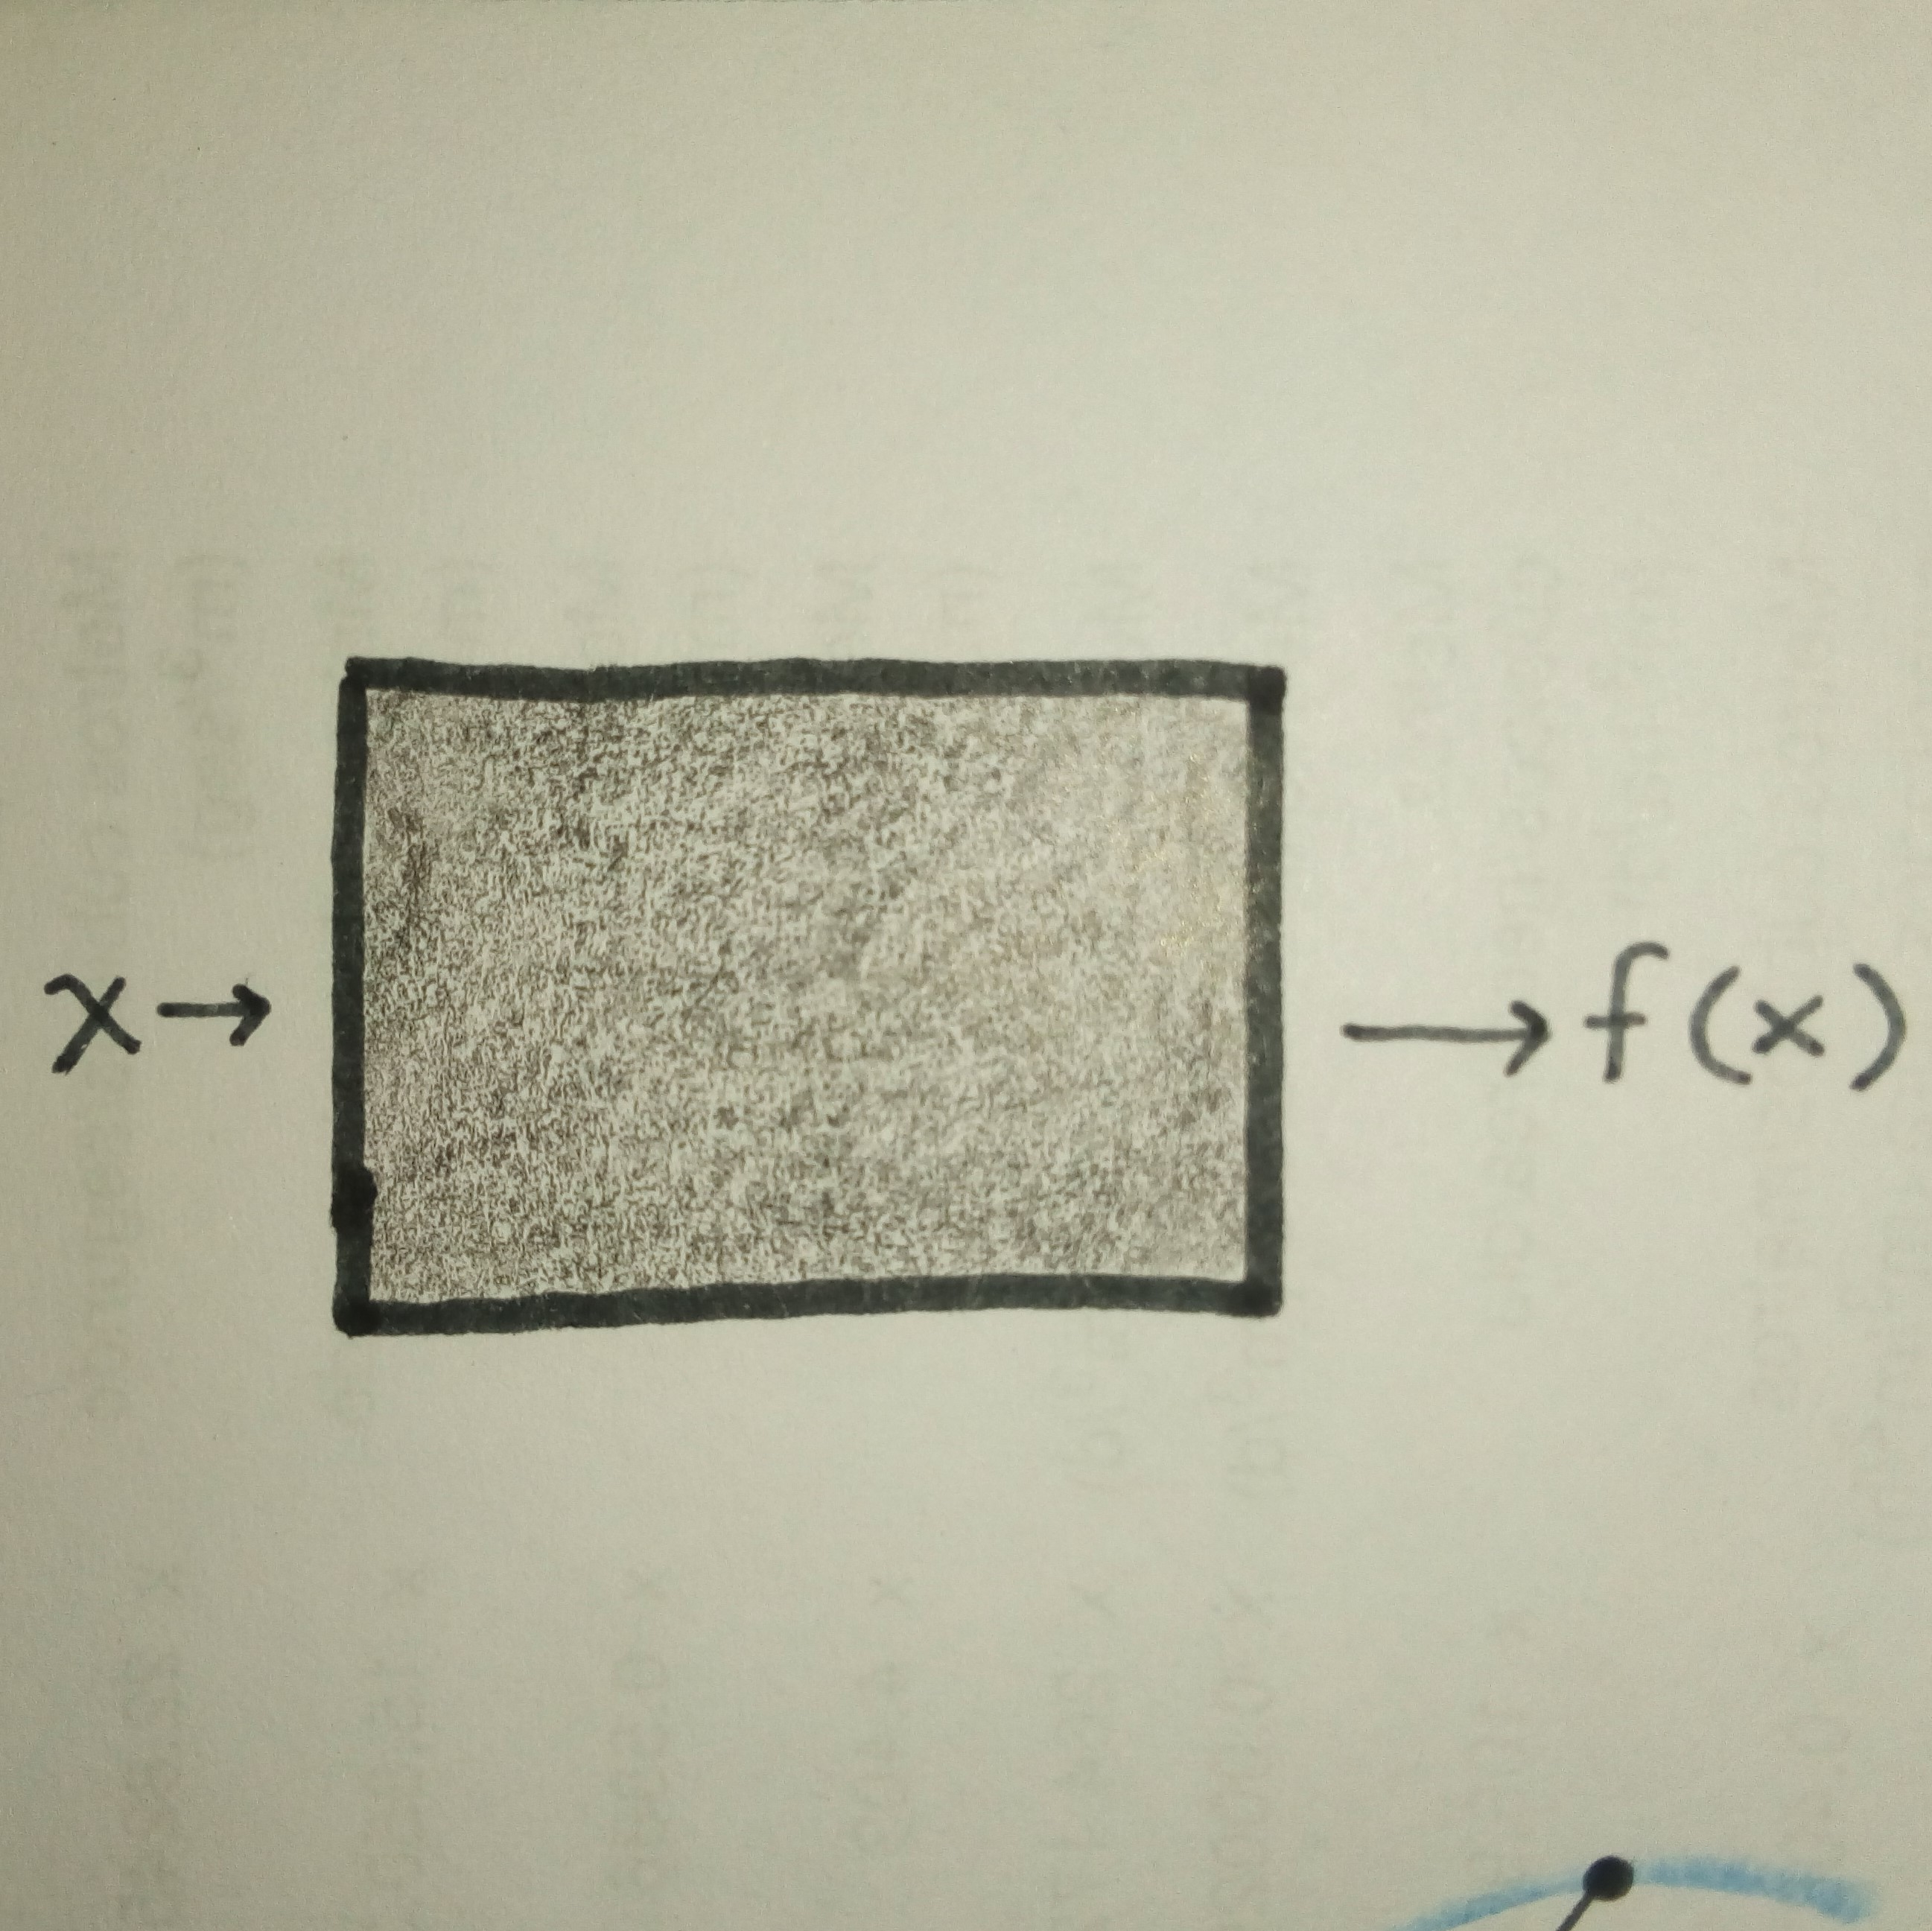
\includegraphics[scale=.05]{imagenes/1.jpg}
\end{center}

\subsection{Bisecci\'on}
Es un algoritmo de b\'usqueda de ra\'ices que trabaja dividiendo el intervalo a la mitad y seccionando el subintervalo que tiene la ra\'iz, y es posible describirlo en los siguientes pasos.\\
\begin{center}
\begin{enumerate}
\item Se eligen los valores limitantes $a$,  $b$ tales que 
\begin{displaymath}
f(a)f(b)\textless0.
\end{displaymath}
\item aproximamos la soluci\'on con la formula del punto medio
\begin{displaymath}
c=\frac{a+b}{2}
\end{displaymath}
\end{enumerate}
\end{center}
\begin{center}
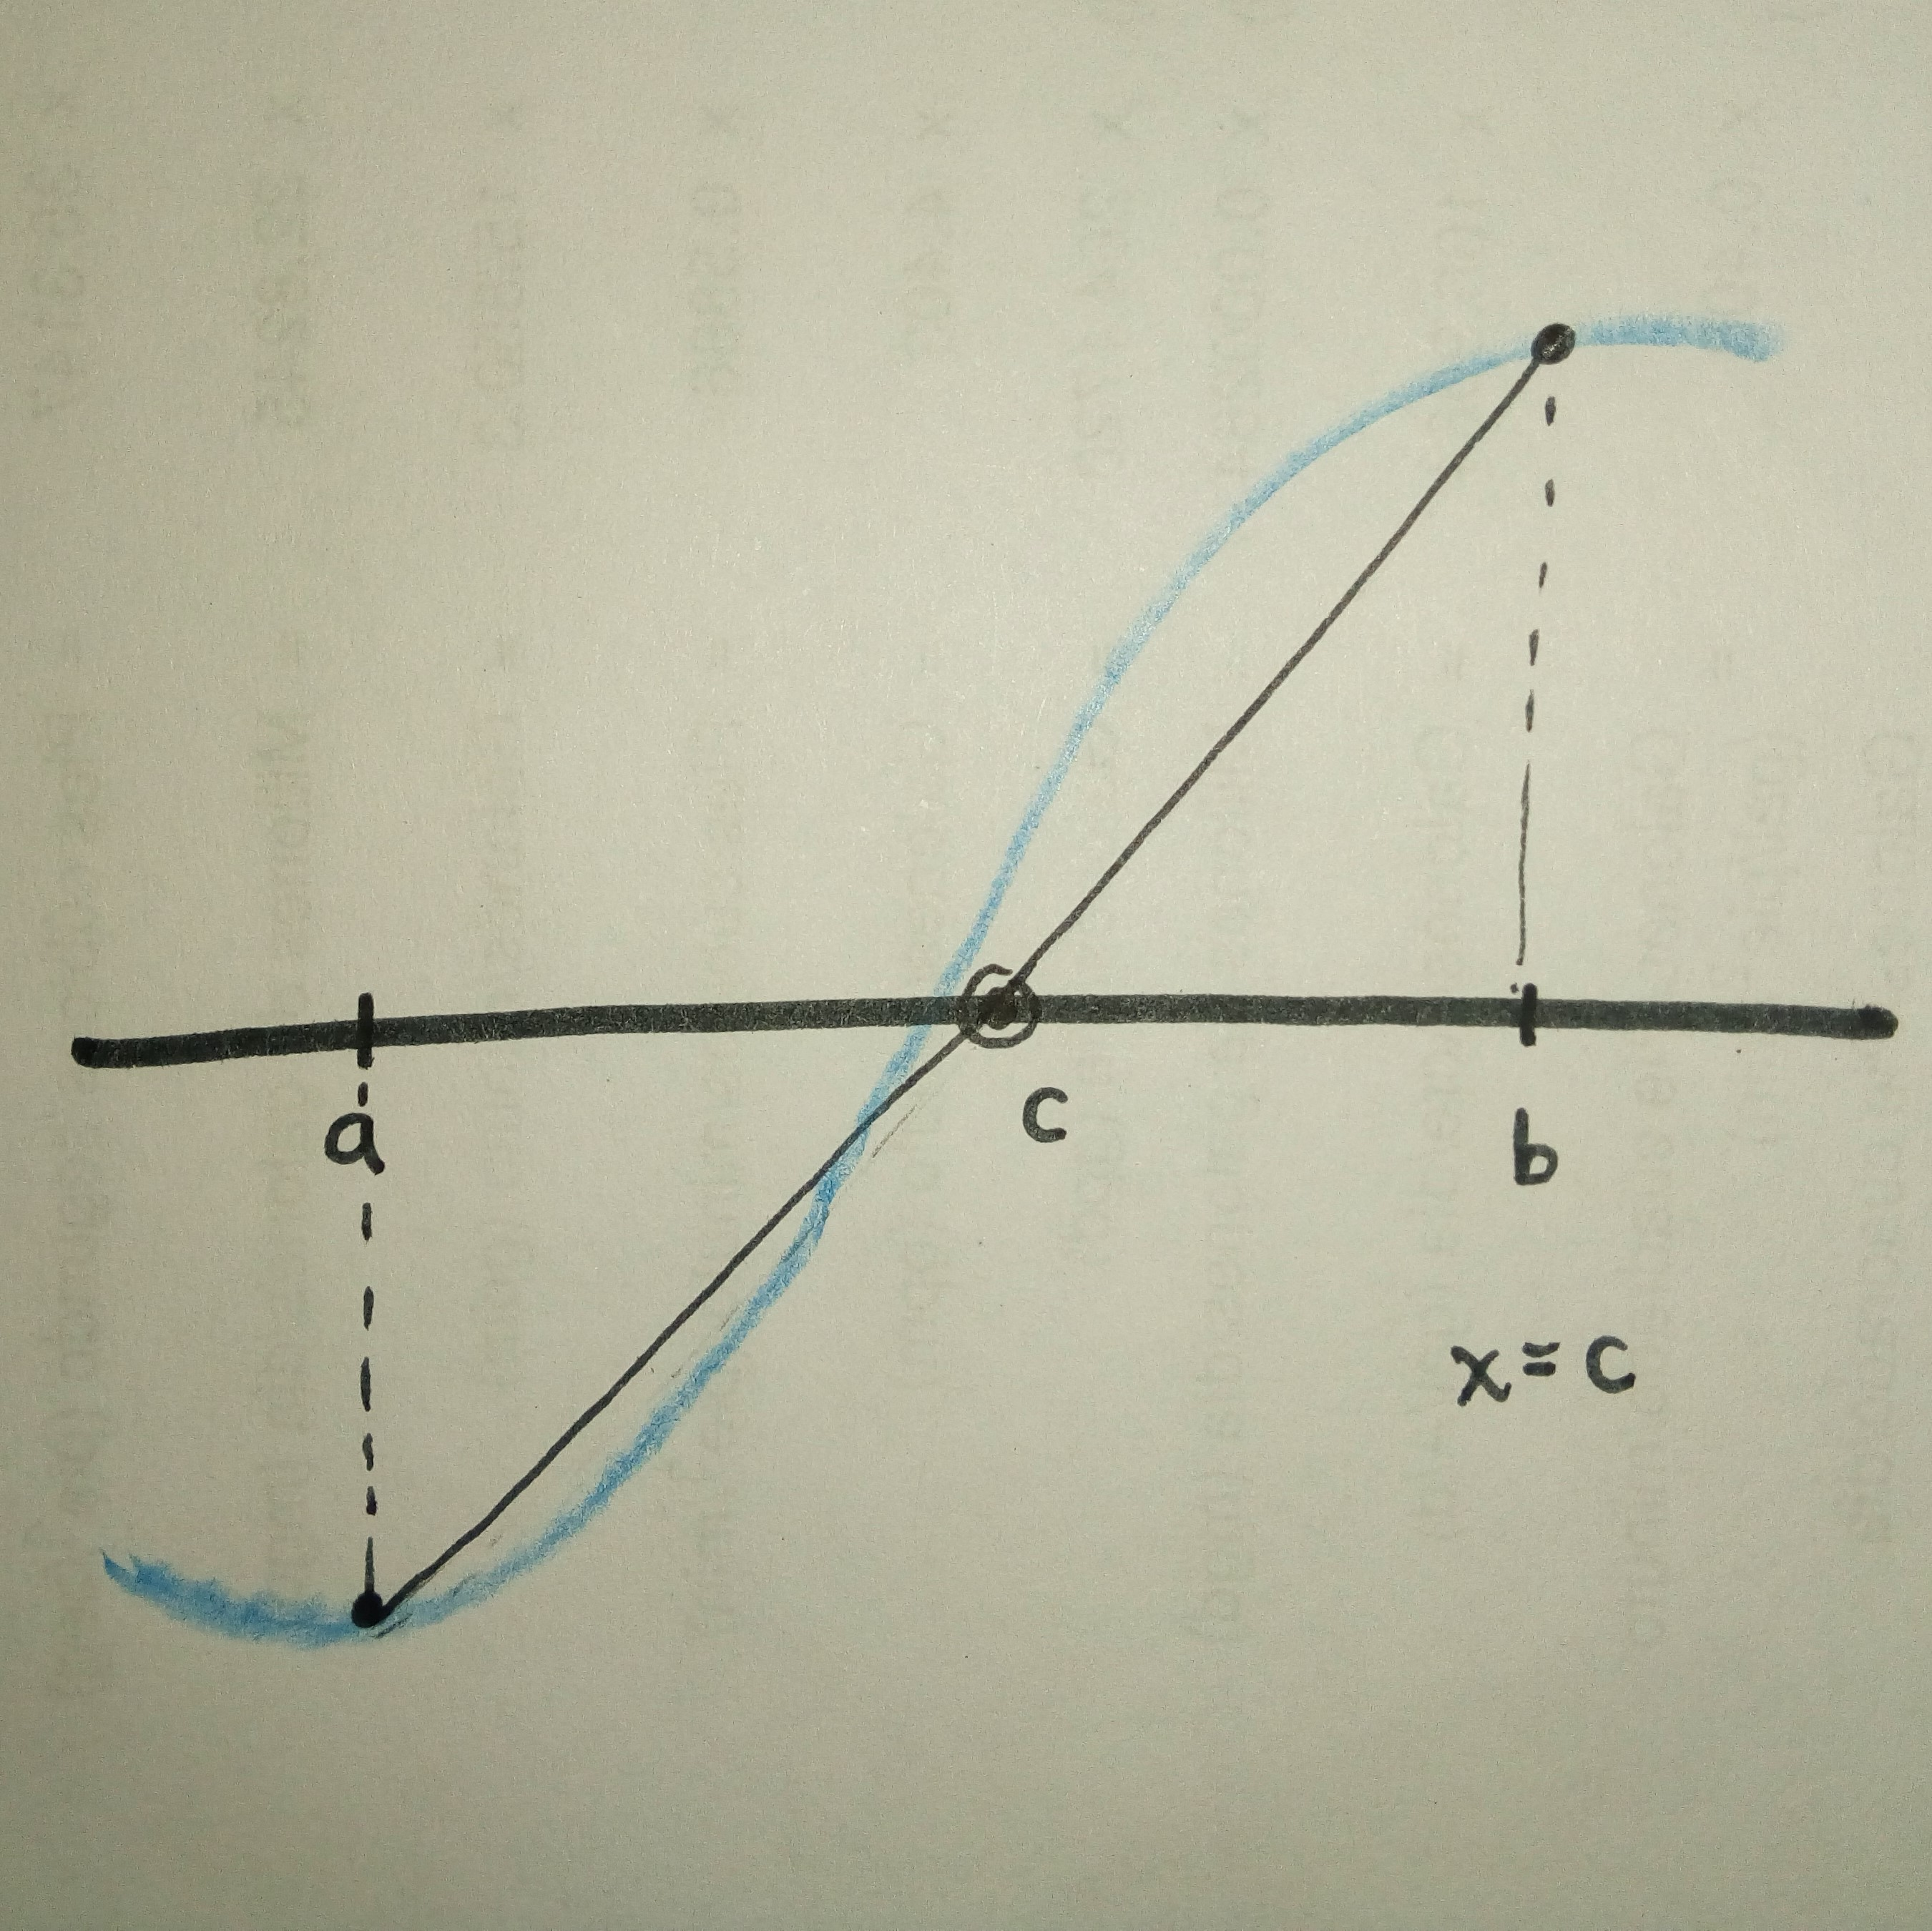
\includegraphics[scale=.05]{imagenes/2.jpg}
\end{center}
%------Algoritmo de bisección-------%
\subsection{M\'etodo de falsa posici\'on o regula-falsi}
Para localizar el punto $c$, se busca la ecuaci\'on de una recta que pasa por los dos puntos de la funci\'on lo que se obtiene es una ra\'iz falsa con una recta el presedimiento se muestra descrito en el siguiente algoritmo.

%-------Algoritmo de falsa posicón-------% 

\section{M\'etodos abiertos}
Son m\'etodos en los que solo necesitamos un valor inicial al que llamamos $x_0$ y son capaces de encontrar ra\'ices tangentes al eje x.

\subsection{M\'etodo de Newton-Raphson}
Consiste en sacas la ecuaci\'on de las tangentes de la funci\'on.
\begin{gather}
y-f(x_o)=f'(x_o)(x-x_0) \\
x_1=x_o-\frac{f(x_1)}{f'(x_1)} \\
x_2=x_1-\frac{f(x_1)}{f'(x_1)} \\
\boxed{x_{k+1}=x_k-\frac{f(x_k)}{f'(x_k)}}
\end{gather}
\begin{center}
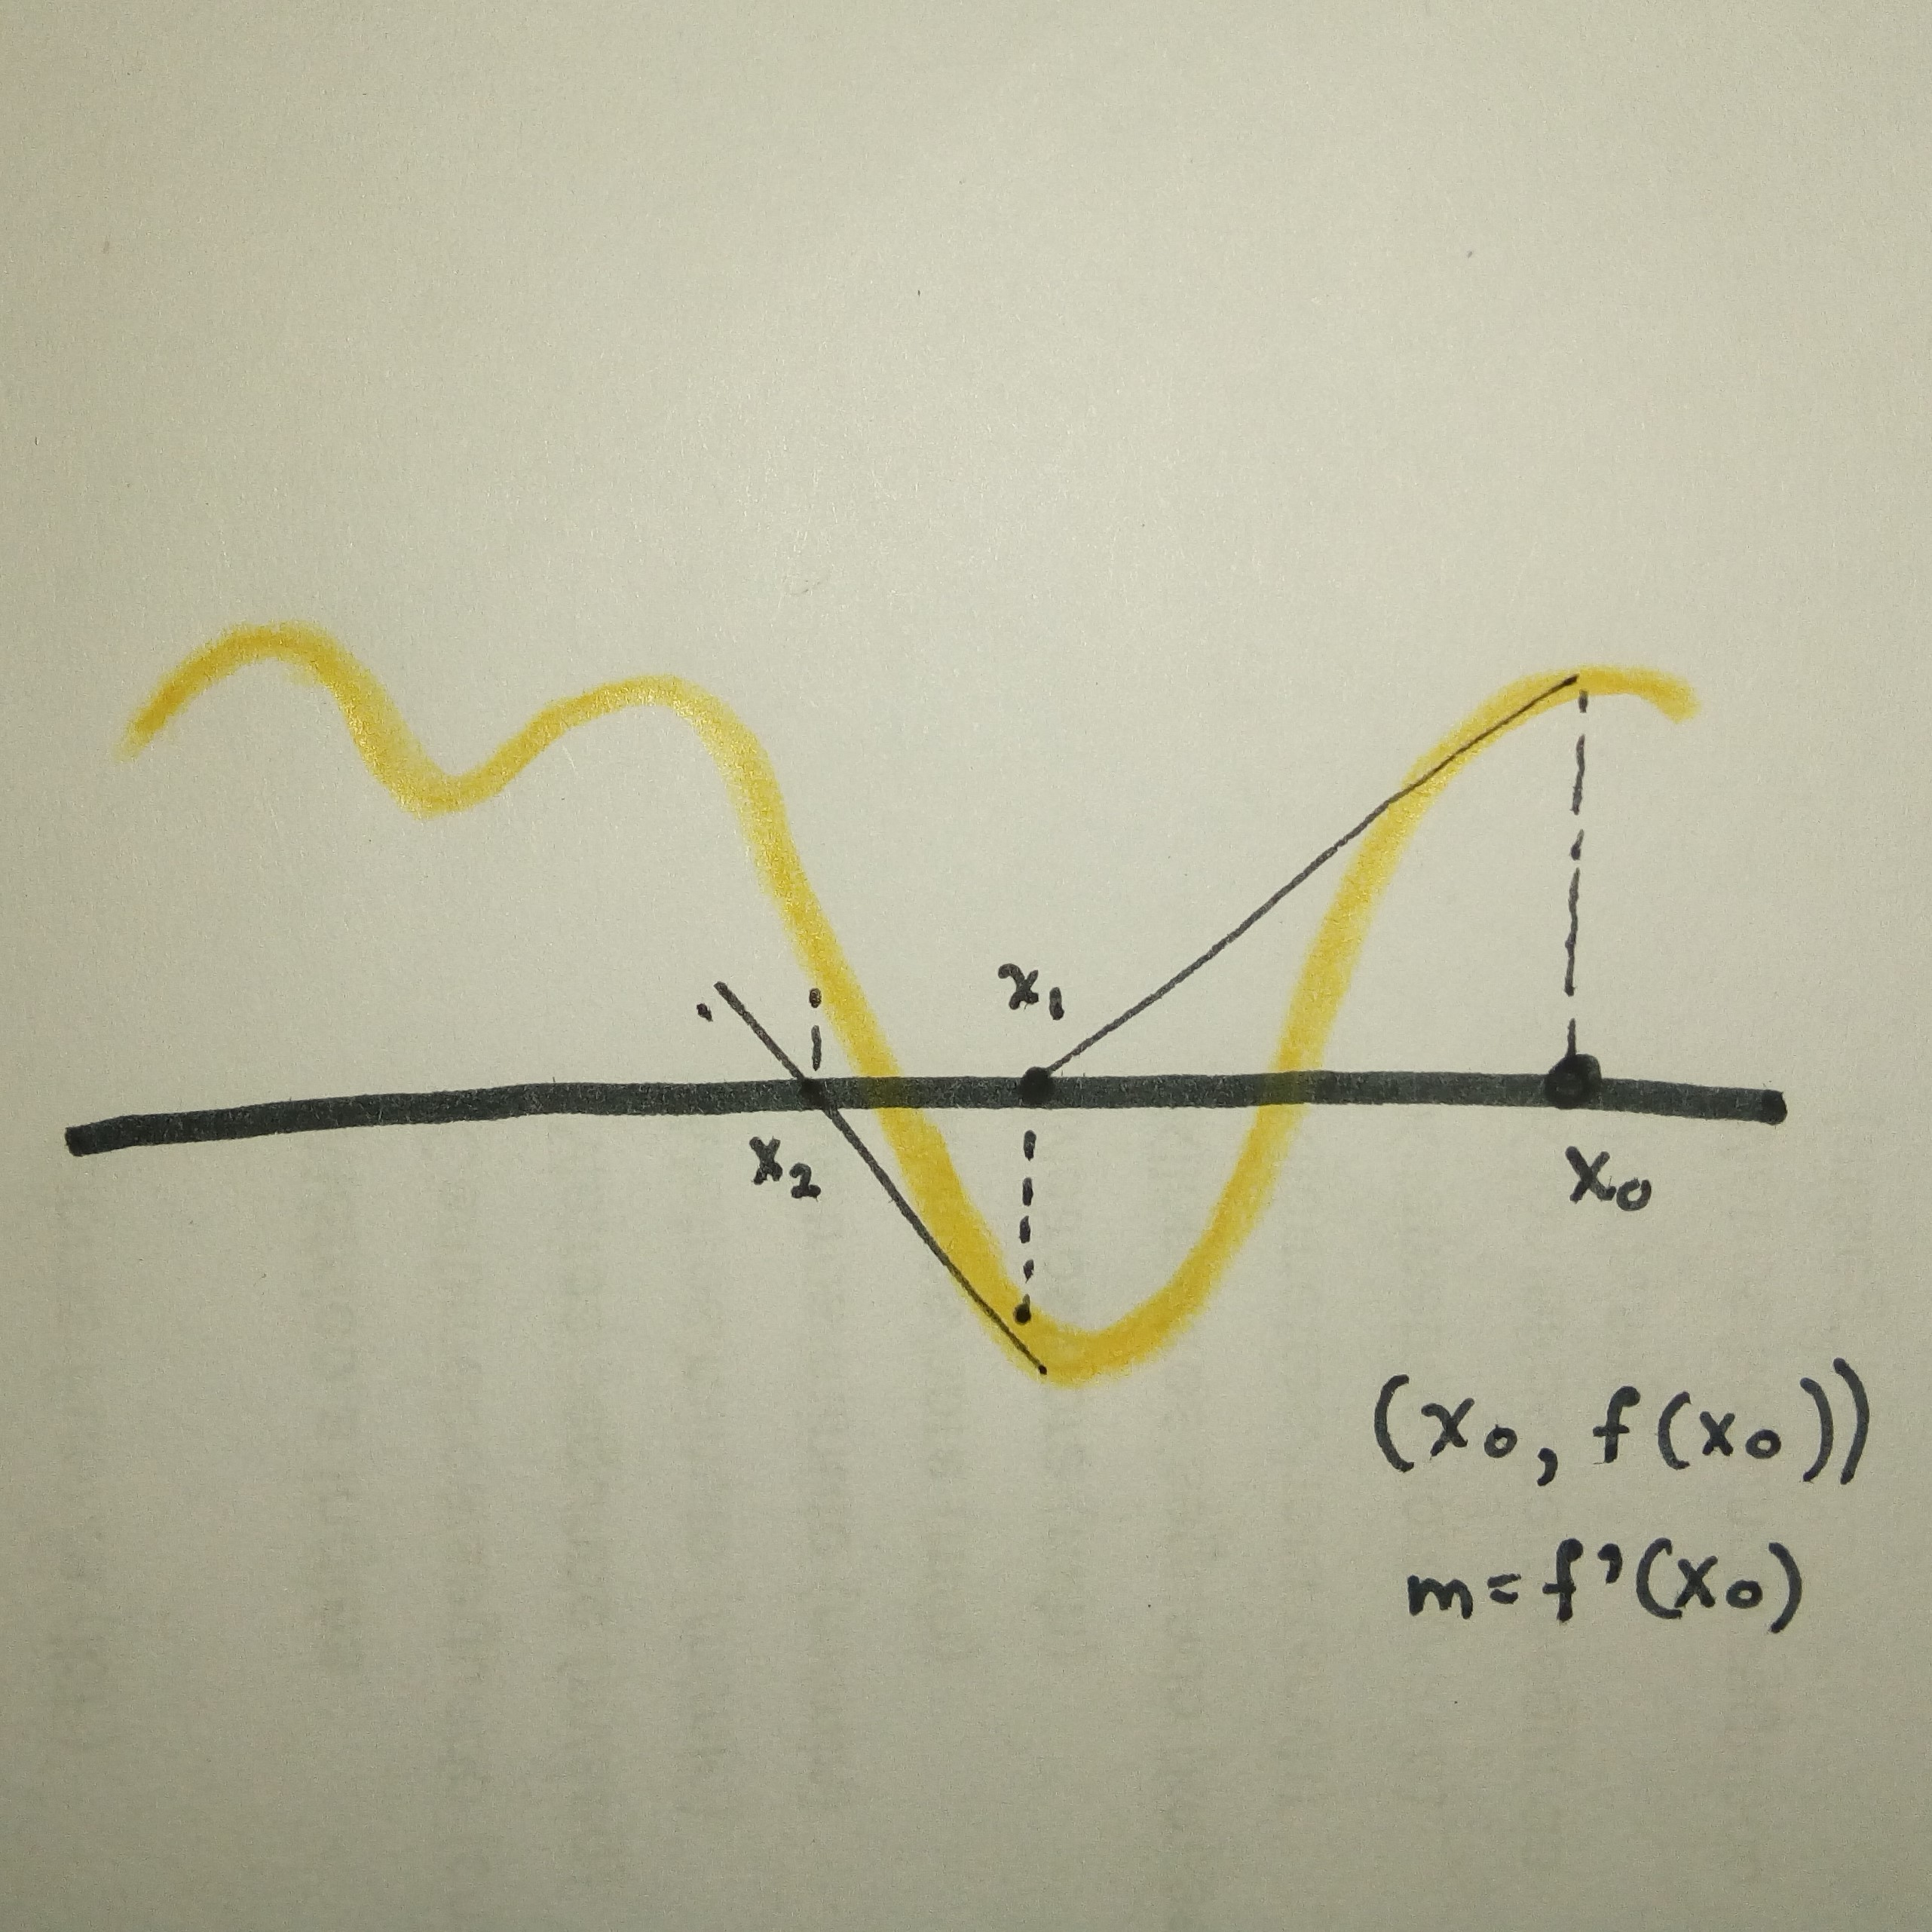
\includegraphics[scale=.05]{imagenes/3.jpg}
\end{center}
\subsubsection*{C\'alculo de error}

\subsection{M\'etodo Secante}
Se trata de un m\'etodo donde se traza una recta secante entro los \'ultimos 2 puntos. Se utilizan derivadas centrales para m\'as precisi\'on y el costo computacional sea menor.
\begin{gather}
\nonumber(x_k,f(x_k+1)) \qquad (x_k,f(x_k))\\
y-f(x_k)=\frac{f(x_k)-f(x_{k-1})}{x_k-x_{k-1}}\\
\boxed{x_{k+1}=x_k-\frac{f(x_k)}{\frac{f(x_k)-f(x_{k-1})}{x_k-x_{k-1}}}}
\end{gather}
\begin{center}
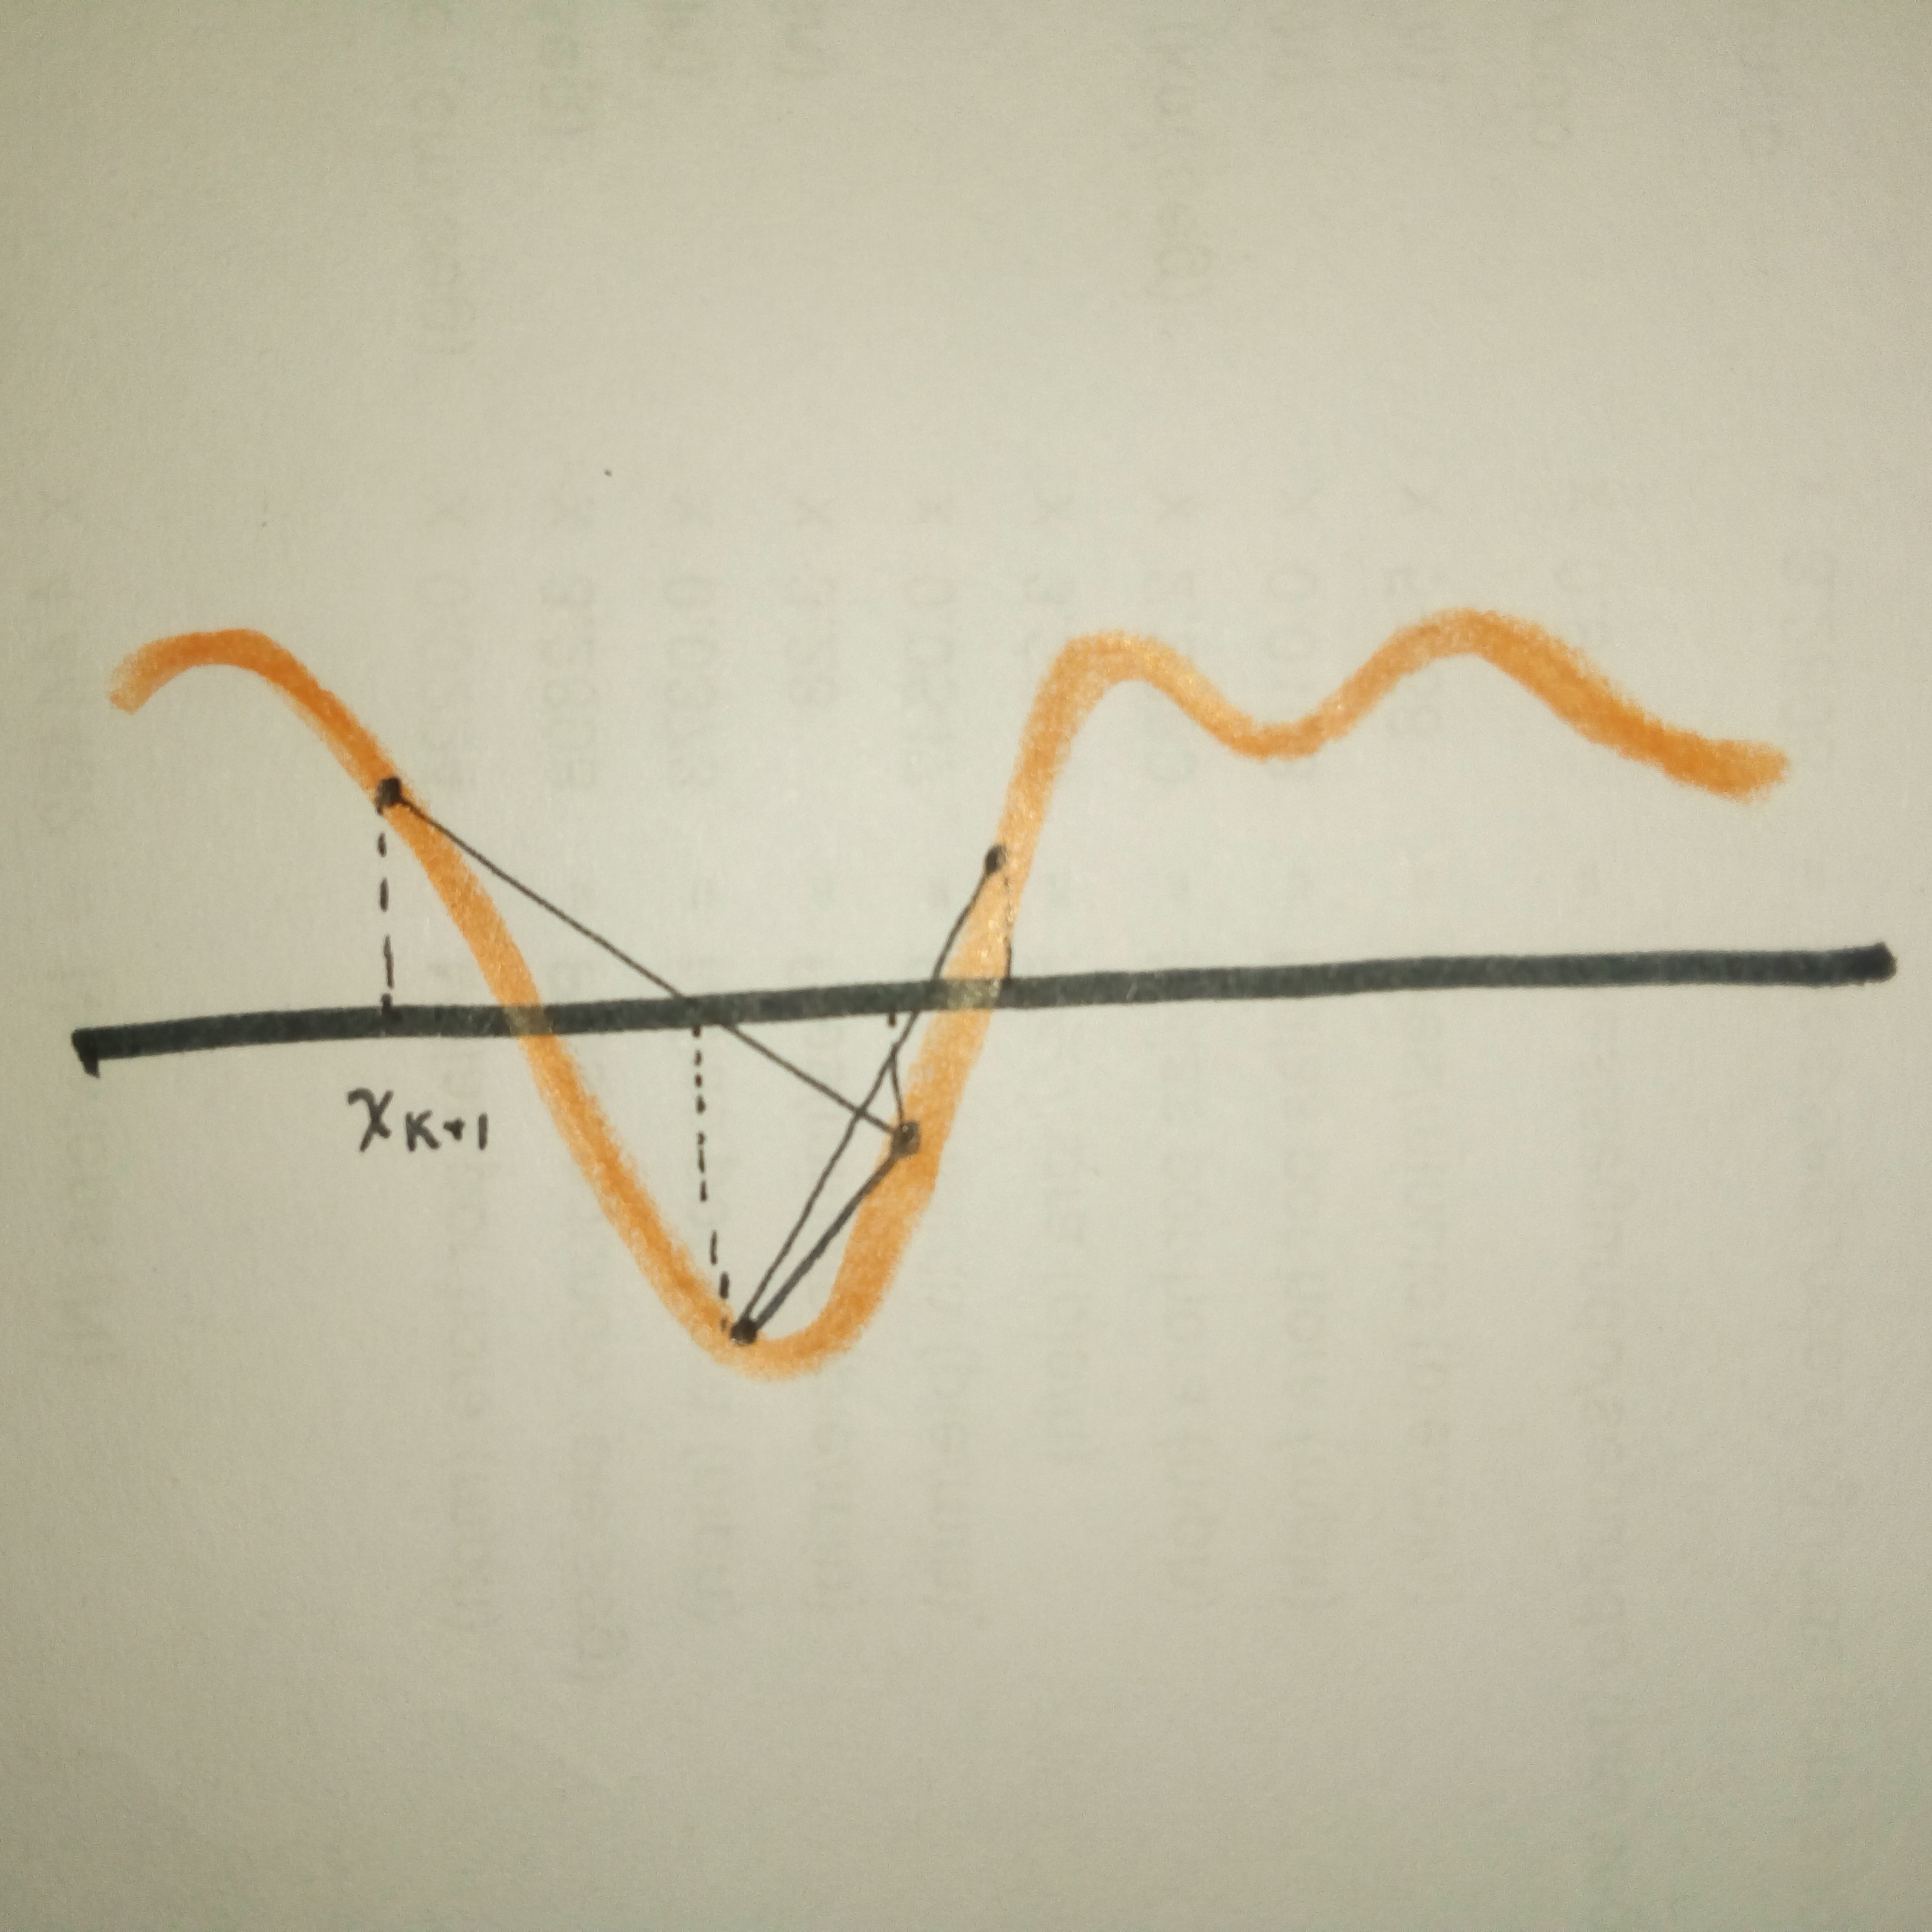
\includegraphics[scale=.05]{imagenes/4.jpg}
\end{center}
\section*{Backtracking}
Es un m\'etodo de b\'usqueda de soluciones exhaustiva sobre grafos dirigidos a ciclos, el cual se acelera mediante poda de ramas poco prometedoras. Es decir se trata de buscar estados soluci\'on del problema. \\
\\
Las condiciones de partida son:
\begin{enumerate}
\item Alcanza la soluci\'on
\item Se alcanzan todos los estados sde soluci\'on
\end{enumerate}
\begin{center}
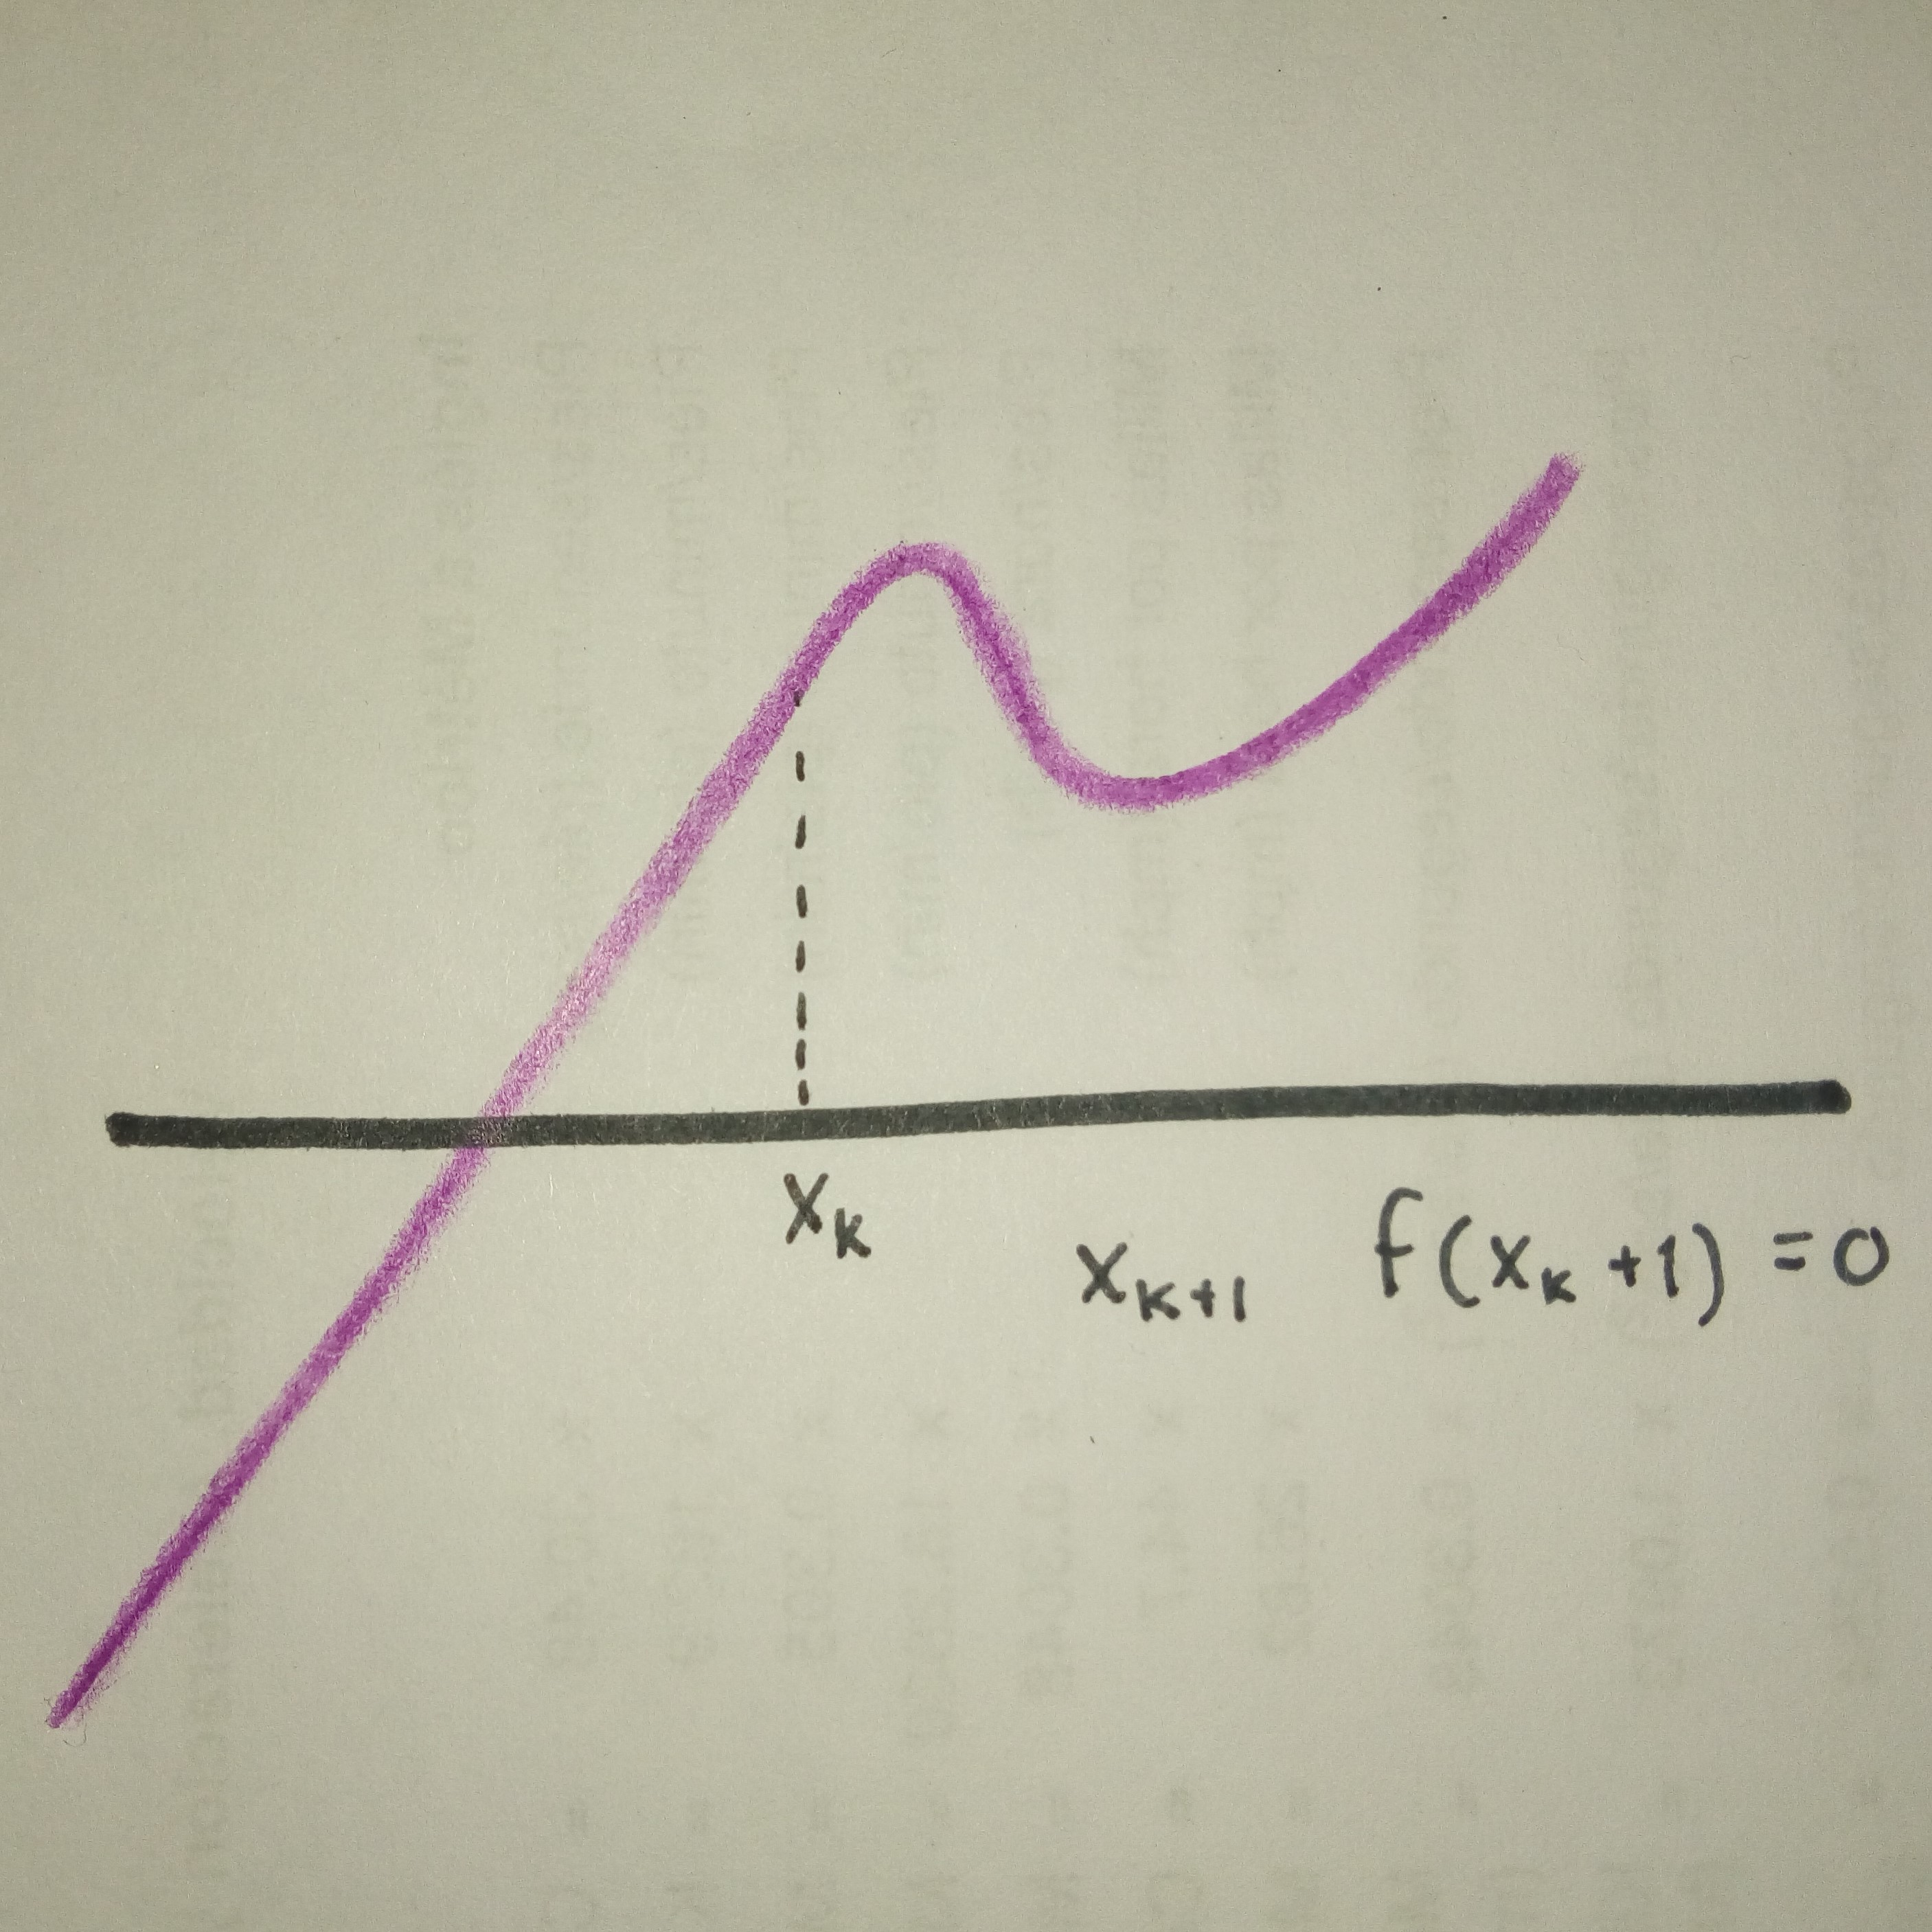
\includegraphics[scale=.05]{imagenes/5.jpg}
\end{center}

\section*{Resumen del c\'apitulo}
Los m\'etodos aqu\'i mostrados son utilizadon para encontrar ra\'ices de funciones y todos llevan al mismo resultado, la gran diferencia esta en el tiempo de computo utilizado para el resultado y la presici\'on de este.\\
\\
\subsection*{Velocidad de convergencia}
La velocida de convergencia que hace referencia al timepo que tarda el ordenador en arrojar un resultado, se muestra en seguida para m\'etodos cerrados y abiertos 
\\
\begin{center}
\begin{tabular}{	c		c	}
M\'etodos & Velocidad de convergencia \\
Bisecci\'on & Lineal [Lento] \\
Falsa posici\'on & Lineal y super lineal \\
Newton-Raphson & Cuadr\'atica [R\'apido] \\
Secante & Cuadr\'atica [R\'apido] \\
\end{tabular}
\end{center}

\subsection*{Iteraciones con y sin backtraking en metodos abiertos}
Si el algoritmo converge en $k$ iteraciones :
\begin{center}
\begin{tabular}{	c		c	}
Newton-Raphson & $2k_1$ \\
Secante & $k_2+1$ \\
Newton-Raphson con B. & $2k_3+Nb_1$ \\
Secante con B. & $k_4+1+Nb_2$
\end{tabular}
\end{center}

\chapter{Soluci\'on de sistemas de ecuaciones}
El objetivo de estos m\'etodos es encontrar un vector soluci\'on para una matriz dada partiendo de la ecuaci\'on $Ax=b$. En este cap\'itulo se describir\'an m\'etodos directos y m\'etodos iterativos. Y lo primero es recordar algunas operaciones y propiedades b\'asicas de las matrices vistas en \'Algebra lineal. 

\section{Operaciones algebr\'aicas con matrices}
\subsection{Suma de matrices}
Es posible sumar dos matrces siempre y cuado sean del mismo tamaño haciendo una adici\'on de sus elementos correspondientes.\\
S\'i $A=[a_{ij}]$ y $B=[b_{ij}]$ son matrices del mismo tamaño $m \times n$, entonces su suma es la matriz de tamaño $m \times n$. \\
\begin{center}
$A+B=[a_{ij}+b_{ij}]$
\end{center}
\subsection{Multiplicaci\'on por un escalar}
Si $A=a_{ij}$ es una matriz de tamaño $m \times n$ y $c$ es un escalar, entonces el multiplo escalar de $A$ por $c$ es la matriz de tamaño $m \times n$ dada por:
\begin{center}
$cA=[ca_{ij}]$
\end{center}  
\subsection{Multiplicaci\'on de matrices}
Si $A=[a_{ij}]$ es una matriz de $m \times n$ y $B=[b_{ij}]$ es una matriz de $m \times p$, entonces el producto $AB$ es una matriz de $m \times p$
\begin{center}
Sea $A=\begin{bmatrix}
a_{11} & a_{12}\\
a_{21} & a_{22}\\
a_{31} & a_{32}
\end{bmatrix}$ y $B=\begin{bmatrix}
b_{11} & b_{12}\\
b_{21} & b_{22}
\end{bmatrix}$ entonces \bigskip \bigskip .
$AB=\begin{bmatrix}
a_{11} & a_{12}\\
a_{21} & a_{22}\\
a_{31} & a_{32}
\end{bmatrix}
\begin{bmatrix}
b_{11} & b_{12}\\
b_{21} & b_{22}
\end{bmatrix}=
\begin{bmatrix}
a_{11}b_{11}+a_{12}b_{21} & a_{11}b_{12}+a_{12}b_{22}\\
a_{21}b_{11}+a_{22}b_{21} & a_{21}b_{12}+a_{22}b_{22}\\
a_{31}b_{11}+a_{32}b_{21} & a_{31}b_{12}+a_{32}b_{22}
\end{bmatrix}$
\end{center}
\subsection{Transpuesta de una matriz}
La transpuesta de una matriz se forma al escribir sus columnas como renglones. Por ejemplo, si $A$ es la matriz de $m \times n$ dada por:
\begin{center}
$A=\begin{bmatrix}a_{11} & a_{12} & a_{13} & \cdots &a_{1n} \\ a_{21} & a_{22} & a_{23} & \cdots & a_{2n}\\ a_{31} & a_{32} & a_{33} & \cdots & a_{3n} \\
\vdots & \vdots & \vdots & \ddots & \vdots\\
a_{m1} & a_{m2} & a_{m3} & \cdots & a_{mn}
\end{bmatrix}$; \bigskip 
 $A^T=\begin{bmatrix}a_{11} & a_{21} & a_{31} & \cdots &a_{m1} \\ a_{12} & a_{22} & a_{32} & \cdots & a_{m2}\\ a_{13} & a_{23} & a_{33} & \cdots & a_{m3} \\
\vdots & \vdots & \vdots & \ddots & \vdots\\
a_{1n} & a_{2n} & a_{3n} & \cdots & a_{mn}
\end{bmatrix}$
\end{center}
\subsection{Matriz sim\'etrica}
Una m\'atriz $A$ es simetrica si $A=A^T$. Partiendo de esta definici\'on, es evidente que una matriz sim\'etrica debe ser cuadrada. Existen cuatro importantes propiedades de matrices simetricas las cuales son:
\begin{enumerate}
\item $(A^T)^T=A$
\item $(A+B)^T=A^T+B^T$
\item $(cA)^T=c(A)^T$
\item $(AB)^T=B^TA^T$
\end{enumerate}
\subsection{Inversa de una matriz}
Una matriz $A$ de $n \times n$ es invertible (o no singular) si existe una matriz $B$ de $n \times n$ tal que $AB=BA=I$, donde $I$ es la matriz identidad de orden n. La matriz $B$ se denomino inversa (multiplicativa) de $A$.\\
Las matrices no cuadradas no tienen inversa.\\
Si A es una matriz invertible, entonces su inversa es \'unica y se denota por $A^{-1}$.
\begin{center}
$AX=I \quad$ Donde $X$ es la matriz inversa.
\end{center}
\subsection{Determinante de una matriz}
El determinante de una matriz est\'a dado por
\begin{center}
$A=\begin{bmatrix}a_{11} & a_{12}\\ a_{21} & a_{22} \end{bmatrix} ; \quad det(A)=|A|=a_{11}a_{22}-a_{21}a_{12}$
\end{center}
El determinante es la diferencia de los products de dos diagonales de la matriz. Si $A$ es una matriz triangular de orden $n$, su determinante es el producto de los elementos en la diagonal principal, $det(A)=|A|=a_{11}a_{22}a_{33}\cdots a_{nm}$
\section{Descomposici\'on matricial}
La descomposici\'on matricial es una forma de factorizaci\'on de matrices en distintas formas para diferentes propositos y resultados. Las principales descomposiciones son descritas a continuaci\'on 
\subsection{Matriz triangular inferior}
Una matriz con una trangulaci\'on inferior la podemos obtener de como producto de la siguiente formula.
\begin{displaymath}
\nonumber x_i=\frac{b_i-\sum_{k=1}^{i-1}a_{ik}x_k}{a_{ii}} 
\end{displaymath}
\begin{center}
$\begin{bmatrix} a_{11} & 0 & 0 & 0 \\
				 a_{21} & a_{22} & 0 & 0 \\
				 a_{31} & a_{32} & a_{33} & 0 \\
				 a_{41} & a_{42} & a_{43} & a_{44}
\end{bmatrix}\begin{bmatrix} x_1 \\
							 x_2 \\
							 x_3 \\
							 x_4 \\
\end{bmatrix} = \begin{bmatrix} b_1 \\
							   b_2 \\
							   b_3 \\
							   b_4 
\end{bmatrix}$
\end{center}
\subsection{Matriz triangular superior}
El contrario de la matris triangular inferior, esta la matriz triangular superior.
\begin{displaymath}
\nonumber x_i=\frac{b_i-\sum_{k=i+1}^{n}a_{ik}x_k}{a_{ii}} 
\end{displaymath}
\begin{center}
$\begin{bmatrix} a_{11} & a_{12} & a_{13} & a_{14} \\
				 0 & a_{22} & a_{23} & a_{24} \\
				 0 & 0 & a_{33} & a_{34} \\
				 0 & 0 & 0 & a_{44}
\end{bmatrix}\begin{bmatrix} x_1 \\
							 x_2 \\
							 x_3 \\
							 x_4 \\
\end{bmatrix} = \begin{bmatrix} b_1 \\
							   b_2 \\
							   b_3 \\
							   b_4 
\end{bmatrix}$
\end{center}
\section{M\'etodos directos}
Los m\'etodos directos se encargan de transforman el sistema original en otro equivalente y f\'acil de reolver.
\subsection{Eliminaci\'on Gaussiana}
\subsection{Factorizaci\'on LU}
\begin{center} $LU \qquad A=LU$ \end{center}
\begin{center} $\begin{bmatrix}
			      a_{11} & a_{12} & a_{13} & a_{14}\\
			      a_{21} & a_{22} & a_{23} & a_{24}\\
			      a_{31} & a_{32} & a_{33} & a_{34}\\
			      a_{41} & a_{42} & a_{43} & a_{44}
			      
\end{bmatrix}= \begin{bmatrix}
			       1 & 0 & 0 & 0\\
			      l_{21} & 1 & 0 & 0\\
			      l_{31} & l_{32} & 1 & 0\\
			      l_{41} & l_{42} & l_{43} & 1
\end{bmatrix} \begin{bmatrix}
                  u_{11} & u_{12} & u_{13} & u_{14}\\
			      0 & u_{22} & u_{23} & u_{24}\\
			      0 & 0 & u_{33} & u_{34}\\
			      0 & 0 & 0 & u_{44}
\end{bmatrix} $
\end{center}
\subsubsection{Doolittle}
La condici\'on para esta factorizaci\'on es:
\begin{center}
$l_{ii}=1$
\end{center}
\begin{displaymath}
L_{ij}=\frac{a_{ij}-\sum_{k=1}^{j-1}l_{ik}u_{kj}}{u_{jj}} \qquad U_{ij}=a_{ij}-\sum_{k=1}^{i-1}l_{ik}u_{kj}
\end{displaymath}
\subsubsection{Crout}
Mientras que para la factorizaci\'on de Crout es:
\begin{center}
$u_{ii}=1$
\end{center} 
\begin{displaymath}
L_{ij}=a_{ij}-\sum_{k=1}^{j-1}L_{ik}U_{kj} \qquad U_{ij}=\frac{a_{ij}-\sum_{k=1}^{j-1}L_{ik}U_{kj}}{L_{ii}}
\end{displaymath}
\subsubsection{Resultados}
\begin{multicols}{2}
\begin{displaymath}a_{11}=u_{11}\end{displaymath}
\begin{displaymath}a_{12}=u_{12}\end{displaymath}
\begin{displaymath}a_{13}=u_{13}\end{displaymath}
\begin{displaymath}a_{14}=u_{14}\end{displaymath}
\begin{displaymath}a_{21}=l_{21}u_{11}\end{displaymath}
\begin{displaymath}l_{21}=\frac{a_{21}}{u_{11}}\end{displaymath}
\begin{displaymath}u_{22}=l_{21}u_{12}+u_{22}\end{displaymath}
\begin{displaymath}a_{23}=a_{22}-l_{21}u_{12}\end{displaymath}
\begin{displaymath}u_{23}=l_{21}u_{13}+u_{23}\end{displaymath}
\begin{displaymath}a_{31}=l_{31}u_{11}\end{displaymath}
\begin{displaymath}l_{31}=\frac{a_{31}}{u_{11}}\end{displaymath}
\begin{displaymath}a_{32}=l_{31}u_{12}+l_{32}u_{22}\end{displaymath}
\begin{displaymath}l_{32}=a_{32}-\frac{l_{31}u_{12}}{u_{22}}\end{displaymath}
\begin{displaymath}a_{33}=l_{31}u_{13}+l_{32}u_{23}+u_{33}\end{displaymath}
\begin{displaymath}u_{33}=a_{33}-(l_{31}u_{13}+l_{32}u_{23})\end{displaymath}
\begin{displaymath}a_{43}=l_{41}u_{13}+l_{42}u_{23}+l_{43}u_{33}\end{displaymath}
\begin{displaymath}l_{43}=\frac{a_{43}-(l_{41}u_{13}+l_{42}u_{23})}{u_{33}}\end{displaymath}
\begin{displaymath}a_{44}=l_{41}u_{14}+l_{42}u_{24}+l_{43}u_{34})\end{displaymath}
\end{multicols}
\subsection*{A es simetrica}
$B^TB$, Da como resultado una matriz sim\'etica. \\
$B^TDB$, Siempre da como resultado una matriz sim\'etrica.
\begin{center}
$\begin{bmatrix}
a_{11} & a_{12} & a_{13} & a_{14} \\
a_{21} & a_{22} & a_{23} & a_{24} \\
a_{31} & a_{32} & a_{33} & a_{34} \\
a_{41} & a_{42} & a_{43} & a_{44} 
\end{bmatrix}=\begin{bmatrix}
l_{11} & 0 & 0 & 0 \\
l_{21} & l_{22} & 0 & 0 \\
l_{31} & l_{32} & l_{33} & 0 \\
l_{41} & l_{42} & l_{43} & l_{44} 
\end{bmatrix}\begin{bmatrix}
l_{11} & l_{12} & l_{13} & l_{14} \\
0 & l_{22} & l_{23} & l_{24} \\
0 & 0 & l_{33} & l_{34} \\
0 & 0 & 0 & l_{44} 
\end{bmatrix} $
\end{center}
\subsection*{Resultados}
\begin{displaymath}a_{11}=l_{11}^2 \qquad l_{11}=\sqrt{a_{11}}\end{displaymath}
\begin{displaymath}a_{43}=a_{34}=l_{31}l_{41}+l_{32}l_{42}+l_{33}l_{43}\end{displaymath}
\begin{displaymath}l_{43}=\frac{a_{43}-(l_{31}l_{41}+l_{32}l_{42})}{l_{33}}\end{displaymath}
\begin{displaymath}a_{44}=l_{41}^2+l_{42}^2+l_{43}^2+l_{43}^2+l_{44}^2\end{displaymath}
\begin{displaymath}l_{44}=\sqrt{a_{44}-l_{41}^2+l_{42}^2+l_{43}}\end{displaymath}
Los m\'etodos que a continuaci\'on se mencionan, son m\'etodos que como condici\'on tienen que la matriz para resolver, debe ser sim\'etrica.
\subsection*{A definida positiva}
Para que una matriz $A$ sea definida positiva si se cumple que $X^TAX>0$ para cualquier vector $X\neq0$
\begin{center}
$A=LDL^T$, tiene soluci\'on param\'etrica
\end{center}
\begin{center}
$\begin{bmatrix}
a_{11} & a_{12} & a_{13} & a_{14} \\
a_{21} & a_{22} & a_{23} & a_{24} \\
a_{31} & a_{32} & a_{33} & a_{34} \\
a_{41} & a_{42} & a_{43} & a_{44} 
\end{bmatrix}=$ \end{center}\begin{center}
$\begin{bmatrix}
1 & 0 & 0 & 0 \\
l_{21} & 1 & 0 & 0 \\
l_{31} & l_{32} & 1 & 0 \\
l_{41} & l_{42} & l_{43} & 1 
\end{bmatrix} \begin{bmatrix}
d_{11} & d_{12} & d_{13} & d_{14} \\
0 & d_{22} & d_{23} & d_{24} \\
0 & 0 & d_{33} & d_{34} \\
0 & 0 & 0 & d_{44} 
\end{bmatrix} \begin{bmatrix}
1 & l_{12} & l_{13} & l_{14} \\
0 & 1 & l_{23} & l_{24} \\
0 & 0 & 1 & l_{34} \\
0 & 0 & 0 & 1
\end{bmatrix}
$\end{center}
\subsection*{Resultados}
\begin{displaymath}a_{34}=a_{43}=a_{11}l_{41}l_{31}+d_{22}l_{42}l_{32}+d_{33}l_{43}\end{displaymath}
\begin{displaymath}l_{43}=\frac{a_{43}-(d_{11}l_{41}l_{31}+d_{22}l_{42}l_{32})}{d_{33}}\end{displaymath}
\begin{displaymath}a_{44}=d_{11}l_{41}^2+d_{22}l_{42}^2+d_{33}l_{43}^2+d_{44}-(d_{11}l_{41}^2+d_{22}l_{42}^2+d_{33}l_{43}^2)\end{displaymath}
\subsection{Factorizaci\'on LLT Cholesky}
\begin{center}
$ A=LL^T$
\end{center}
La factorizaci\'on de Cholesky adem\'as de requerir una matriz simetrica, debe ser definida positiva y cabe mencionar que este m\'etodo tiene una soluci\'on \'unica.
\subsubsection*{Para los que estan en la diagonal}
\begin{center}
$L_{ii}=\sqrt{a_{ii}-\sum_{k=1}^{i-1}l_{ik}^2}$
\subsubsection*{Para los que estan fuera de la diagonal}
\begin{center}
$L_{ij}=L^T_{ji}=\frac{a_{ij}+\sum_{k=1}^{j-1}l_{ik}l_{jk}}{l_{jj}}$
\end{center}
\end{center}
\subsection{Factorizaci\'on LDLT}
\begin{center}
$ A=LDL^T $
\end{center}
\begin{center}
$L_{ij}=\frac{a_{ij}-\sum_{k=1}^{j-1}d_{kk}l_{ik}l_{jk}}{d_{jj}} \qquad d_{ii}=a_{ii}-\sum_{k=1}^{i-1}d_{kk}l_{ik}^2$
\end{center}
\section{M\'etodos iterativos }
\begin{center}
$Ax=b=f(x)=0$
\end{center}
Estos m\'etodos parten de un vector inicial $x^o$, y la modificaci\'on mediante un esquema repetitivo de c\'alculo hasta llegar a la soluci\'on buscada.
\subsection{M\'etodo de punto fijo}
\begin{center}
$f(x)=0\qquad \rightarrow \qquad g(x)=x$ \\
$x_0$ \\
$x_1=g(x_0)$ \\
$\vdots$ \\
$x_{k+1}=g(x_k)$
\end{center}
Este m\'etodo consiste en separar un sistema lineal y distribuir para tener m\'as valores de "$x$".
\begin{center}
$A=(L+D+U)$
\end{center}
D\'onde $D$ es una matriz diagonal y las matrices $L$ y $U$ son triangulares.
\begin{center}
$(L+D+U)x=b$ \\
$(L+U)x+Dx=b$ \\
$D^{-1}[Dx=b-(L+U)x]$ \\
$x=D^{-1}[b-(L+U)x]$ \\
\end{center}
\subsection{M\'etodo de Jacobi}
Es un m\'etodo sensible al orden en que se encuentran acomodadas las ecuaciones. Remplaza el vector hasta que est\'a completo y se necesita que converja r\'apido para poder comparar el rendimiento con un m\'etodo directo.
\begin{center}
$x^o$ \end{center}
\begin{center}$x^{k+1}=D^{-1}[b-(L+U)x^k]$\end{center}
\begin{center}$\begin{bmatrix}
x_1 \\ x_2 \\ x_3 \\ x_4 
\end{bmatrix}^{k+1}=\left(\begin{bmatrix}
\frac{1}{a_{11}} & 0 & 0 & 0 \\
0 & \frac{1}{a_{22}} & 0 & 0 \\
0 & 0 & \frac{1}{a_{33}} & 0 \\
0 & 0 & 0 & \frac{1}{a_{44}}
\end{bmatrix}\begin{bmatrix}
b_1 \\ b_2 \\ b_3 \\ b_4
\end{bmatrix}-\begin{bmatrix}
0 & a_{12} & a_{13} & a_{14} \\
a_{21} & 0 & a_{23} & a_{24} \\
a_{31} & a_{32} & 0 & a_{34} \\
a_{41} & a_{42} & a_{43} & 0
\end{bmatrix}^k\right)$
\end{center}
\begin{displaymath}
x_i^{k+1}=\frac{1}{a_{ii}}(b_i\sum_{j=i+1}^{i-1}a_{ij}k_j^k-\sum _{j=i+1}^na_{ij}x_j^k)
\end{displaymath}
\\
\begin{displaymath}
\frac{\parallel x^{k+1}-x^k \parallel}{max(\parallel x^{k+1} \parallel, \parallel x^k \parallel)}>e_1
\end{displaymath}
\subsubsection*{Condici\'on de convergencia}
Es necesario que la matriz $A$ sea diagonalmente dominante, \'osea que, en cada rengl\'on de $A$, se debe cumplir que: 
\begin{displaymath}
|a_{ii}|\geq \sum_{j=1,j\neq i}^n |a_{ij}| \qquad |a_{ii}|\gg |a_{ij}|
\end{displaymath}
%Algoritmo de Jacobi%
\subsection{M\'etodo de Gauss-Seidel}
Este es un m\'etodo de convergencia r\'apido. Va reutilizando las mismas "$x$".
\begin{center}
$(L+D+U)x=b$ \\
$(L+D)x^{k+1}=b-Ux^k$ \\
$D^{-1}(Dx^{k+1}=b-[x^{k+1}-Ux^k)]$ \\
$x^{k+1}=D^{-1}[b-Lx^{k+1}-Ux^k]$ 
\end{center}
\begin{center}$x^{k+1}=D^{-1}[b-(L+U)x^k]$\end{center}
\begin{center}$\begin{bmatrix}
x_1 \\ x_2 \\ x_3 \\ x_4 
\end{bmatrix}^{k+1}=\begin{bmatrix}
\frac{1}{a_{11}} & 0 & 0 & 0 \\
0 & \frac{1}{a_{22}} & 0 & 0 \\
0 & 0 & \frac{1}{a_{33}} & 0 \\
0 & 0 & 0 & \frac{1}{a_{44}}
\end{bmatrix}\left(\begin{bmatrix}
b_1 \\ b_2 \\ b_3 \\ b_4
\end{bmatrix}-\begin{bmatrix}
0 & 0 & 0 & 0 \\
a_{21} & 0 & 0 & 0 \\
a_{31} & a_{32} & 0 & 0 \\
a_{41} & a_{42} & a_{43} & 0
\end{bmatrix}\begin{bmatrix}
x_1 \\ x_2 \\ x_3 \\ x_4\\
\end{bmatrix}^{k+1}-\begin{bmatrix}
0 & a_{12} & a_{13} & a_{14} \\
0 & 0 & a_{23} & a_{24} \\
0 & 0 & 0 & a_{34} \\
0 & 0 & 0 & 0
\end{bmatrix} \begin{bmatrix}
x_1 \\ x_2 \\ x_3 \\ x_4
\end{bmatrix}^k \right)$
\end{center}
\begin{displaymath}
x_1^{k+1}=\frac{1}{a_{11}}[b_1-(a_{12}x_2^k+a_{13}x_3^k+a_{14}x_4^k)]
\end{displaymath}
\begin{displaymath}
x_2^{k+1}=\frac{1}{a_{22}}[b_2-a_{21}x_1^{k+1}-(a_{23}x_3^k+a_{24}x_4^k)]
\end{displaymath}
\begin{displaymath}
x_i^{k+1}=\frac{1}{a_{ii}}(b_i-\sum_{j=1}^{i-1}a_{ij}x_j^{k+1}-\sum_{j=i+1}^{n}a_{ij}x_j^k)
\end{displaymath}
\subsubsection*{Condici\'on de convergencia}
En la mayoria de los casos, si: $|a_{ii}|\gg|a_{ij}|$ en cada regi\'on sin que sea necesario.
\subsection{M\'etodo de Gauss-Seidel con relajaci\'on (SOR)}
Es una aplica\'ion de Gauss-Seidel, converge m\'as r\'apido, pero no siempre se cumple, depende del valor de $W$. Donde $W$ es un valor param\'etrico.\\
Se basa en el m\'etodo de triangulaci\'on $W\in[0,2]$
\begin{displaymath}
x^{k+1}=(1-W)x^k+Wx_{GS}^{k+1}
\end{displaymath}
*GS hace referencia al metodo Gauus-Seidel simple
\begin{displaymath}
x_{i}^{1-W}x_i^k+\frac{W}{a_{ii}}\left[ b_i-\sum_{j=1}^{i-1}a_{ij}x_j^{k+1}-\sum_{j=i+1}^{n}a_{ij}x_j^k\right]
\end{displaymath}
La $W$ mas usual es $W=1.5$

\subsection*{Comceptos de Gradientes}

\subsubsection*{Gradiente de un campo escalar}
Sea $F:U\leq R^3\rightarrow R$ un campo escalar, $g$ sean
\begin{displaymath}
\frac{\delta f}{\delta x}; \frac{\delta f}{\delta y}; \frac{\delta f}{\delta z}
\end{displaymath}
Las derivadas parciales de $f$ (es decir, derivar respecto a una variable manteniendo las otras como constantes).\\
Entonces el gradiente conjugado de $f$ es:
\begin{displaymath}
grad(f)=\left(\frac{\delta f}{\delta x},\frac{\delta f}{\delta x},\frac{\delta y}{\delta z}\right)
\end{displaymath}

El gradiente apunta en la direci\'on en la que la derivada direccional de la funci\'on f es m\'axima, y su m\'odulo en un punto es el valor de esta derivada direccional en ese punto. \\
Se anula en los puntos de inflexi\'on de la funci\'on $f$.\\
El gradiente convierte en un campo escalar en un campo vectorial.

\subsubsection*{Divergencia de un campo escalar}
Sea $F:U\leq R^3\rightarrow R^3$, $F=(F_1,F_2,F_3)$ un campo vectorial. Entonces la divergencia de $F$ es:
\begin{displaymath}
div(F)=\frac{\delta}{\delta x}F_1+\frac{\delta}{\delta y}F_2+\frac{\delta}{\delta z}F_3
\end{displaymath}
La divergencia convierte un campo vectorial en un campo escalar.
\subsection*{Rotacional de un campo vectorial}
Sea $F:U\leq R^3\rightarrow R^3$, $F=(F_1,F_2,F_3)$ un campo vectorial. Entonces; el rotacional de $F$ es:
\begin{displaymath}
vot(F)=\left(\frac{\delta F_3}{\delta y}-\frac{\delta F_2}{\delta z},\frac{\delta F_1}{\delta z}-\frac{\delta F_3}{\delta x},\frac{\delta F_1}{\delta y} \right)
\end{displaymath}
o tambi\'en se puede calcular como el siguiente determinante, (teniendo en cuenta que i,j,k son la coordenada a la que corresponden):
\begin{displaymath}
\left| \begin{matrix}
i & j & k \\
\frac{\delta}{\delta x} & \frac{\delta}{\delta y} & \frac{\delta}{\delta z} \\
F_1 & F_2 & F_3

\end{matrix} \right|
\end{displaymath}

\subsubsection*{Propiedades del gradiente, divergencia y rotacional}
\begin{enumerate}
\item $rot(grad(F))=0$
\item $div(rot(F)=(grad(f)xF+f.rot(F))=0$
\item $rot(f.F)=$
\item $div(f.F)=f.div(F)+grad(f).F$
\end{enumerate}

\subsection*{Valores m\'aximos y m\'inimos}
Una funci\'on de dos variables tiene un m\'aximo relativo en $(a,b)$ si $f(x,y)\leq f(a,b)$ cuando $(x,y)$ esta cerca de $(a,b)$. El n\'umero $f(a,b)$ recibe el nombre de valor m\'aximo relativo. Si $f(x,y)\leq f(a,b)$ cuando $(x,y)$ est\'a cerca de $(a,b)$, entonces $f(a,b)$ es un m\'inimo relativo en $(a,b)$ y $f(a,b)$ es un valor m\'aximo relativo.\\
Si lo anterior se cumple para todos los puntos $(x,y)$ en el dominio de $f$, entonces $f$ tiene un m\'aximo absoluto o un m\'aximo absoluto en $(a,b)$\smallskip 
Teorema\\
Si $f$ tiene un m\'aximo o un m\'aximo relativo en $(a,b)$ y las derivadas parciales de primer orden existen all\'i, entonces $Fx(a,b)=0$ y $Fy(a,b)=0$.\\
Un punto $(a,b)$ se llama punto cr\'itico de $f$ si $fx(a,b)=0$ y $fy(a,b=0)$ o si una de estas derivadas parciales no existe.

\section*{Analisis de sensibilidad de los sistemas lineales}
\begin{displaymath}
\begin{bmatrix}
a_{11} & a_{12} \\
a_{21} & a_{22}
\end{bmatrix}\begin{bmatrix}
x \\ y
\end{bmatrix}\begin{bmatrix}
b_1 \\ b_2
\end{bmatrix}
\end{displaymath}
\begin{center}
$a_{11}x+a_{12}y=b_1$\\
$\frac{a_{11}}{a_{12}}x+y=\frac{b_1}{b_2}$\\
$\frac{a_{21}}{a_{22}}x+y=\frac{b}{a_{22}}$
\end{center}
\subsection*{Sistemas mal condicionados}
\begin{center}
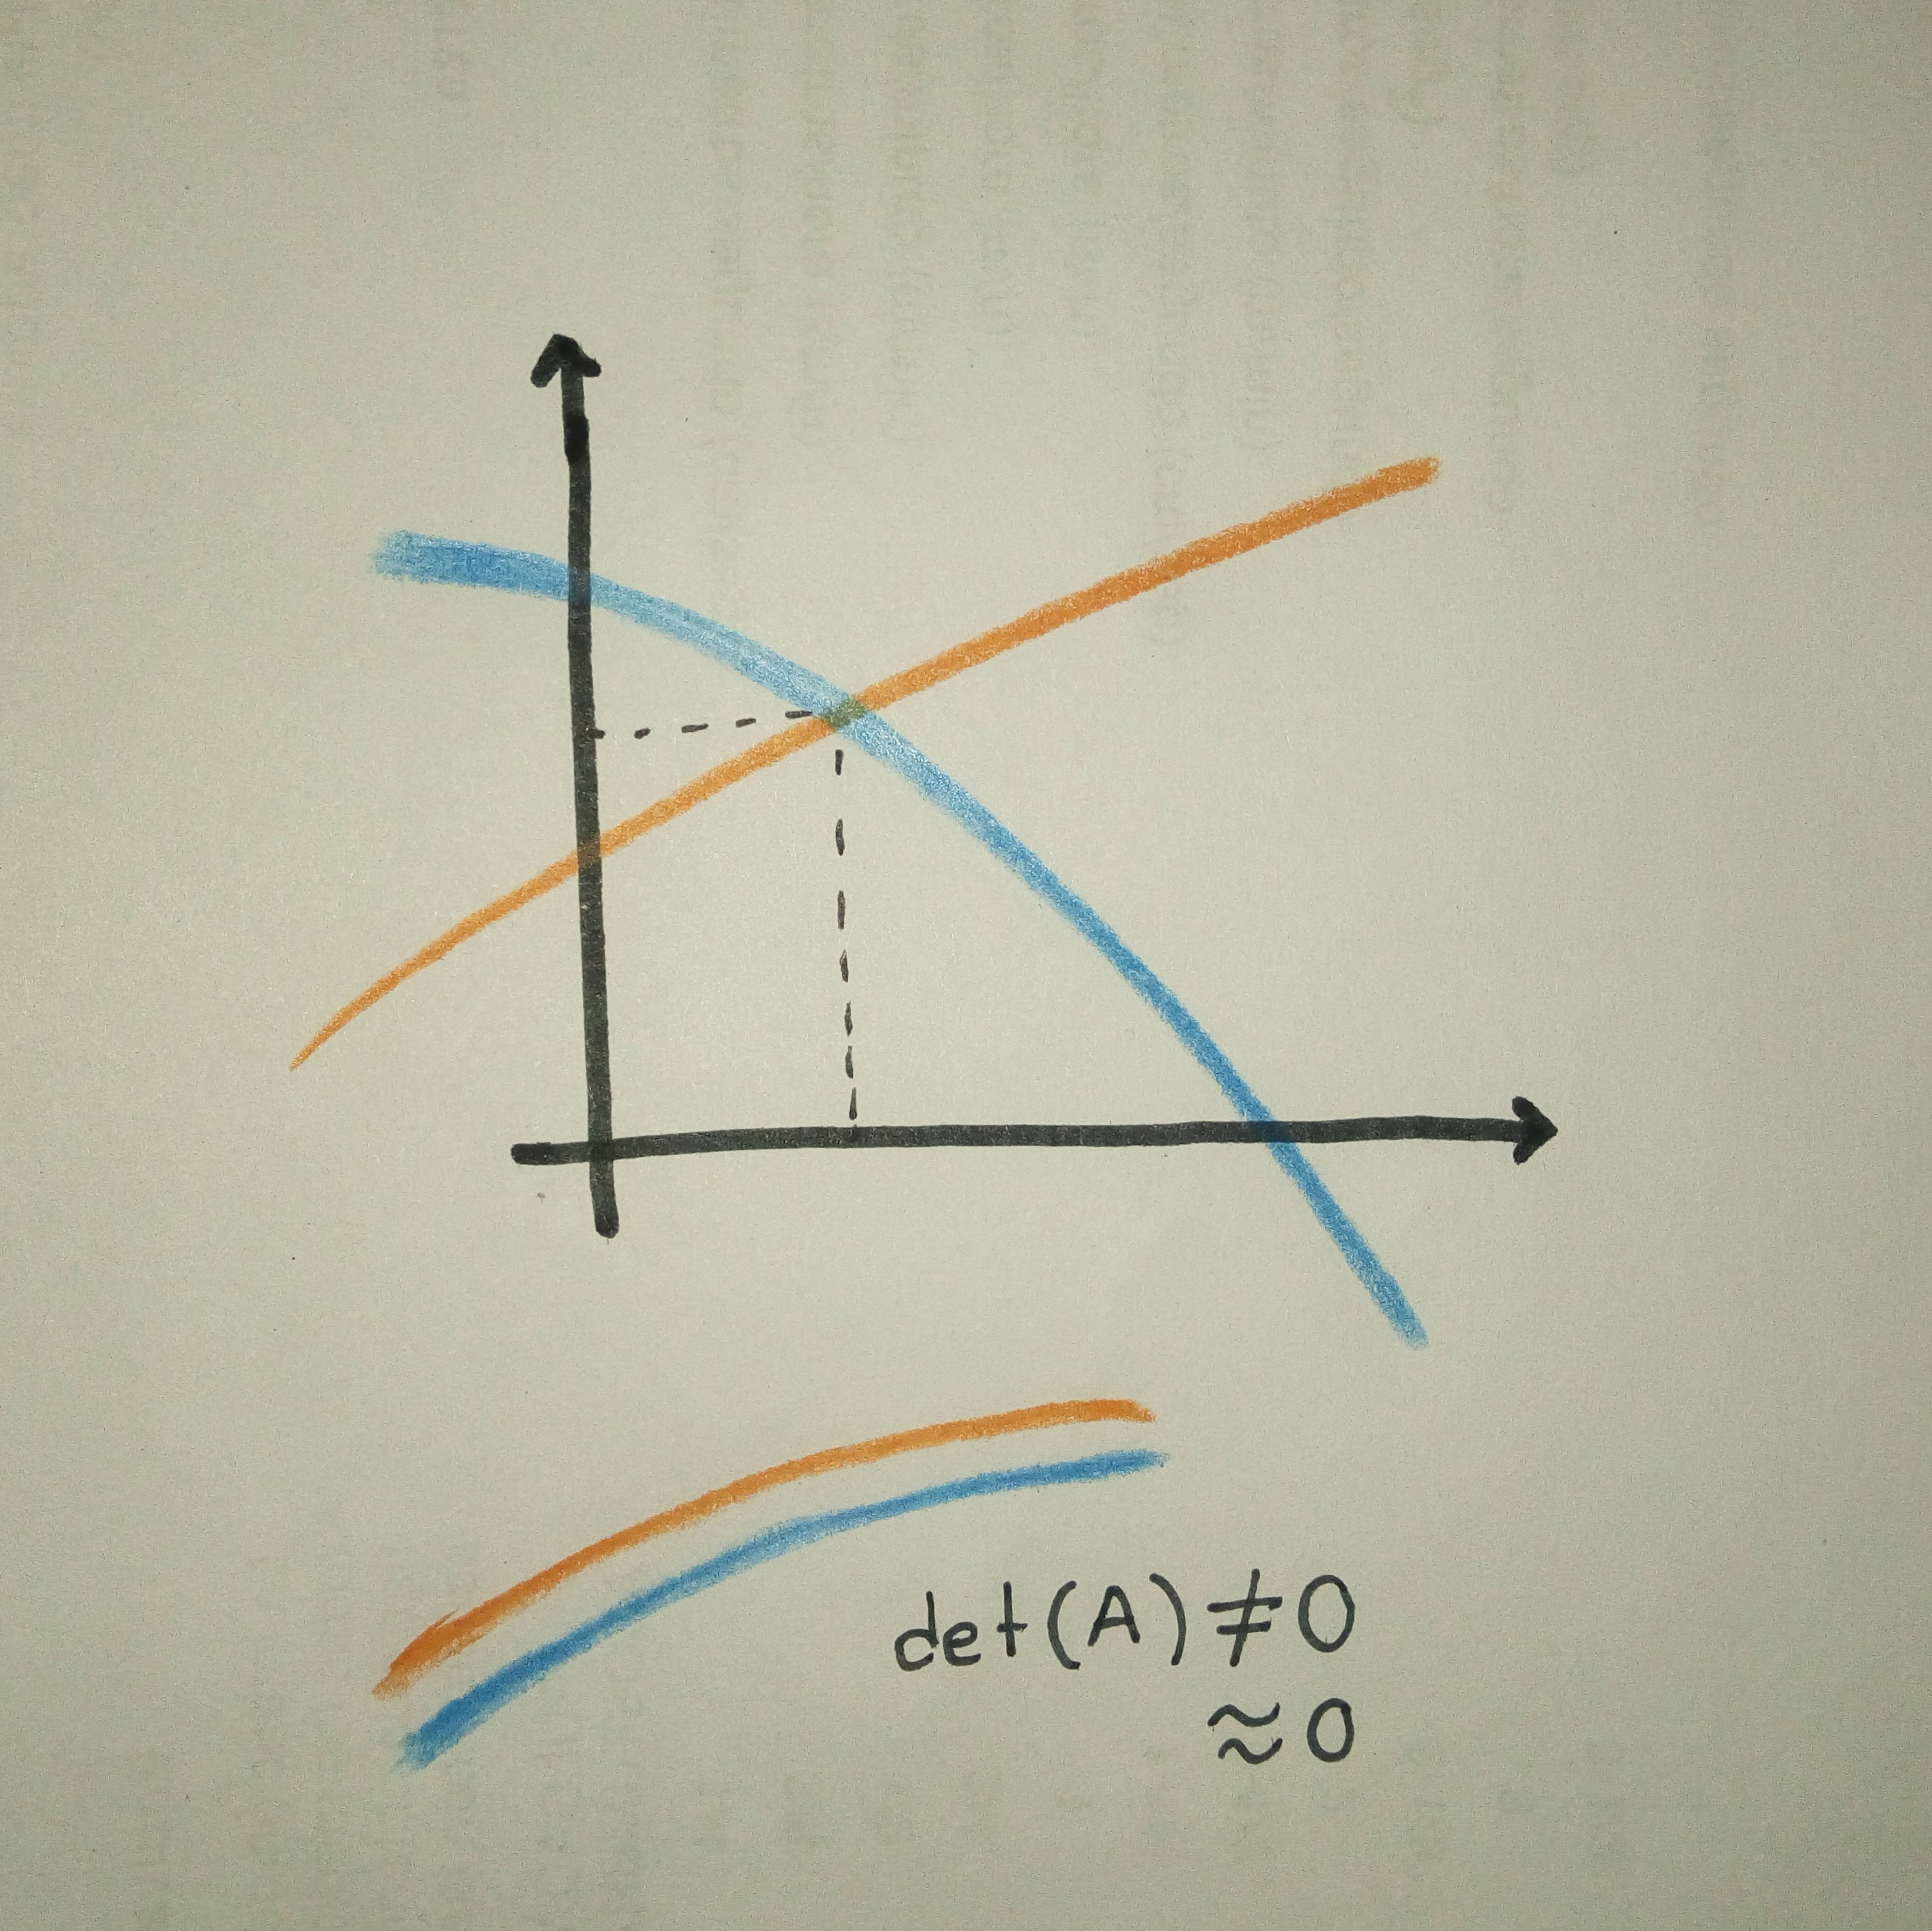
\includegraphics[scale=.05]{imagenes/6.jpg}
\end{center}
En este tipo de casos estos sistemas son muy sensibles ante errores nu\'ericos.
\subsubsection*{N\'umero de condici\'on de una matriz cuadrada}
\begin{displaymath}
Cond(A)=\parallel A \parallel \bullet \parallel A^{-1} \parallel
\end{displaymath}
Para alguna norma matricial.
\begin{center}
$|V|_e=\sqrt{\sum V_i^2}$\\
$|V|_1=max|V_i|$
\end{center}
\begin{itemize}
\item Norma Eucliniana o Norma de Frobenius\\
\begin{center}
$\parallel A \parallel _1 = \sqrt{\sum \sum a_i^2}$
\end{center}
\item Norma 1 \'o columna-suma\\
\begin{center}
$\parallel A \parallel = max_{1\leq j\leq n}\sum_{i=1}^{n}|a_{ij}|$
\end{center}
\item Norma $\infty$ \'o renglon-suma\\
\begin{center}
$\parallel A \parallel _{\infty} = max_{1\leq i\leq n}\sum_{j=1}^{n}|a_{ij}|$\end{center}
\item Norma z \'o norma espectral\\
Cuando el n\'umero de condici\'on es muy pequeño quiere decir que los sistemas no estan tan mal condicionados y son proporcionakes. 
\item Condici\'on A \begin{displaymath}
cond(A)=\frac{\parallel \Delta x \parallel }{\parallel x \parallel}\leq \frac{\parallel \Delta A \parallel }{\parallel A \parallel} 
\end{displaymath}
$\Delta x:$ Es el cambio en la soluci\'on $x$ de sistema lineal debido a los errores num\'ericos. \\
$\Delta A:$ Es el cambio en la matriz del sistema debido a la aritm\'etica inexacta de las computadoras.
\begin{center}
$Cond(A)\nsim 1$\\
$Cond(A)\ggg 1 $
\end{center}
\end{itemize} 
\subsection{M\'etodo de Gradiente conjugado}
\subsubsection{Gradiente conjugado}
El gradiente se ubica donde la pendiente es m\'as grande (Es decir la direcci\'on en la cu\'al se tienen la m\'axima pendiente). Los puntos cr\'iticos son donde el gradiente es 0.\\
$z=f(x,g)$\\
\begin{displaymath}
\nabla f=\begin{bmatrix}
\frac{\delta f}{\delta x}
\frac{\delta f}{\delta y}
\end{bmatrix}
\end{displaymath}
%Diagrama del gradiente%
$f(x,y)$\\
$\nabla f=0$\\
$\nabla ^2f$ \\
$det(\nabla ^2f)$
\begin{itemize}
\item $>0 minimo$
\item $=0 silla$
\item $<0 maximo$
\end{itemize}
$f'(x)=0$ indica pendiente\\
$f''(x)$
\begin{itemize}
\item $>0 minimo$
\end{itemize}
$\nabla f=\begin{bmatrix}
\frac{\delta f}{\delta x} \\
\\
\frac{\delta f}{\delta y} 
\end{bmatrix} \qquad \nabla ^2f=\begin{bmatrix}
\frac{\delta ^2f}{\delta x^2} & \frac{\delta ^2f}{\delta x\delta y}\\
\\
\frac{\delta ^2f}{\delta y\delta x} & \frac{\delta ^2f}{\delta y^2} 
\end{bmatrix}_{Matriz Gaussiana} $ 
\begin{center}
\begin{displaymath}
x=\begin{bmatrix}
x \\ y
\end{bmatrix}
\end{displaymath}
$x^{k+1}= x^k+\alpha_kP_k$\\
%Diagramita de gráfica%
Todos estos puntos van a estar detrtminados por $x+\alpha P$, donde $x$ es la posici\'on inicial y $\alpha P$ la distancia al valor inicial\\
\end{center}
\subsubsection{An\'alisis del m\'etodo}
Es un m\'etdo de convergen en "n" iteraciones con aritm\'etica exacta.\\
$Ax=b$\\
Si A es sim\'etrica y $det(A)>0$, el problema es equivalente a\\
\begin{center}
$min\quad \phi(x)=\frac{1}{2}x^TAx-x^Tb$\\ $\nabla\phi(x)=0$
\end{center}
\begin{displaymath}
\frac{1}{2}\begin{bmatrix}
x & y \end{bmatrix}\begin{bmatrix}
a_{11} & a_{12} \\ a_{21} & a_{22}\end{bmatrix}\begin{bmatrix}
x\\y \end{bmatrix}-\begin{bmatrix}
x & y \end{bmatrix}\begin{bmatrix}
b_1 \\ b_2 \end{bmatrix}
\end{displaymath}

\begin{displaymath}
\frac{1}{2}\begin{bmatrix}
x & y \end{bmatrix}\begin{bmatrix}
a_{11}x & a_{12}y \\ a_{21}x & a_{22}y\end{bmatrix}- xb_1 - yb_2
\end{displaymath}
\begin{displaymath}
\phi(x)=\frac{1}{2}a_{11}x^2+a_{12}xy+\frac{1}{2}a_{22}y^2-xb_1-yb_2
\end{displaymath}
\begin{displaymath}
\frac{\delta\phi}{\delta x}=a_{11}x+a_{12}y-b_1
\end{displaymath}
\begin{displaymath}
\frac{\delta\phi}{\delta y}=a_{21}x+a_{22}y-b_2
\end{displaymath}
\begin{displaymath}
\boxed{\nabla\phi(x)=Ax-d}
\end{displaymath}
$x^o$\\
$x^{k+1}=x^k+\alpha_kP_k$\\
$f(\alpha)=\phi(x^k+\alpha P)$\\
$f'(\alpha)=P\cdot\nabla\phi(x^k+\alpha P)=P^T[A(x^k+\alpha P)-b]$\\
$f'(\alpha)=P^TAx^k+\alpha P^TAP-P^Tb=0$
\begin{displaymath}
\alpha=\frac{-P^TAx^k+P^Tb}{P^TAP}=\frac{-P^T(Ax^k-b)}{P^TAP}=\frac{-P^T\nabla\phi(x^k)}{P^TAP}
\end{displaymath}
\begin{center}
$\nabla\phi(x^k)=Ax^k-b$\\
$x^{k+1}=x^k+\alpha_kP_k$
\end{center}
\begin{displaymath}
\alpha_k=\frac{P_k^T\nabla\phi(x^k)}{P_k^TAP_k}
\end{displaymath}
Para una matriz sim\'etrica $A$ con $det(A)\leq 0$, existe un conjunto de $n$ direcciones linealmente independientes que cumplen la siguiente propiedad
\begin{displaymath}
P_i^TAP_j\rightarrow\quad =0\quad si\quad i\leq j ;\qquad \leq 0 \quad si\quad i=j
\end{displaymath}
y se llaman direcciones conjugadas.
\begin{displaymath}
P_k^TA(x^*-x^o=\sigma_oP_o+\sigma_1P_1+\sigma_2P_2+\cdots+\sigma_{n-1}P_{n-1})
\end{displaymath}
\begin{displaymath}
P_k^TA(x^*-x^o)=\sigma_oP_k^TAP_o+\sigma_1P_k^TAP_1+\sigma_2P_k^TAP_2+\sigma_kP_k^TAP_k+\cdots+\sigma_{n-1}P_k^TAP_{n-1}
\end{displaymath}
\begin{displaymath}
P_k^TA(x^*-x^o)=\sigma_kP_k^TAP_k
\end{displaymath}
\begin{displaymath}
\boxed{\sigma_k=\frac{P_kA(x^*-x^o)}{P_k^TAP_k}}
\end{displaymath}
\begin{displaymath}
\nabla\phi(x^k)=Ax^k-b
\end{displaymath}
\begin{displaymath}
x^{k+1}=x^k+\alpha_kP_k
\end{displaymath}
\begin{displaymath}
\alpha_k=\frac{-P_k^T\nabla\phi(x^k)}{P_k^TAP_k}
\end{displaymath}
\begin{displaymath}
P_k^TA(x^k=x^o+\alpha_oP_o+\alpha_1P_1+\alpha_2P_2+\cdots+\alpha_{k-1}P_{k-1})
\end{displaymath}
\begin{displaymath}
P_x^TAx^k=P_kAx^o+\alpha_oP_k^TAP_o+\alpha_1P_k^TAP_1+\cdots+\alpha_{k-1}P_k+AP_{k-1}
\end{displaymath}
\begin{displaymath}
P_k^TAx^k=P_kAx^o
\end{displaymath}
\begin{displaymath}
P_k^TA(x^k-x^o)=0
\end{displaymath}
\begin{displaymath}
\sigma_k=\frac{P_k^T(b-Ax^k)}{P_k^TAP_k}
\end{displaymath}
\begin{displaymath}
\sigma_k=\frac{-P_k^T(Ax^k-b)}{Pk^TAP_k}
\end{displaymath}
\\
\begin{displaymath}
\sigma_k=\frac{P_k^T(b-Ax^k)}{P_k^TAP_k}-\frac{P_k^T(Ax^k-b)}{P_k^TAP_k}
\end{displaymath}
\begin{displaymath}
P_o=-r_o
\end{displaymath}
\begin{displaymath}
P_{k-1}^TA(P_k=-r_k+B_kP_{k-1})
\end{displaymath}
\begin{displaymath}
P_{k-1}^TAP_k=-P_{k-1}^TAr_k+B_kP_{k-1}^TAP_{k-1}
\end{displaymath}
\begin{displaymath}
B_k=\frac{P_{k-1}^TAr_k}{P_{k-1}^TAP_{k-1}}
\end{displaymath}
\begin{center}
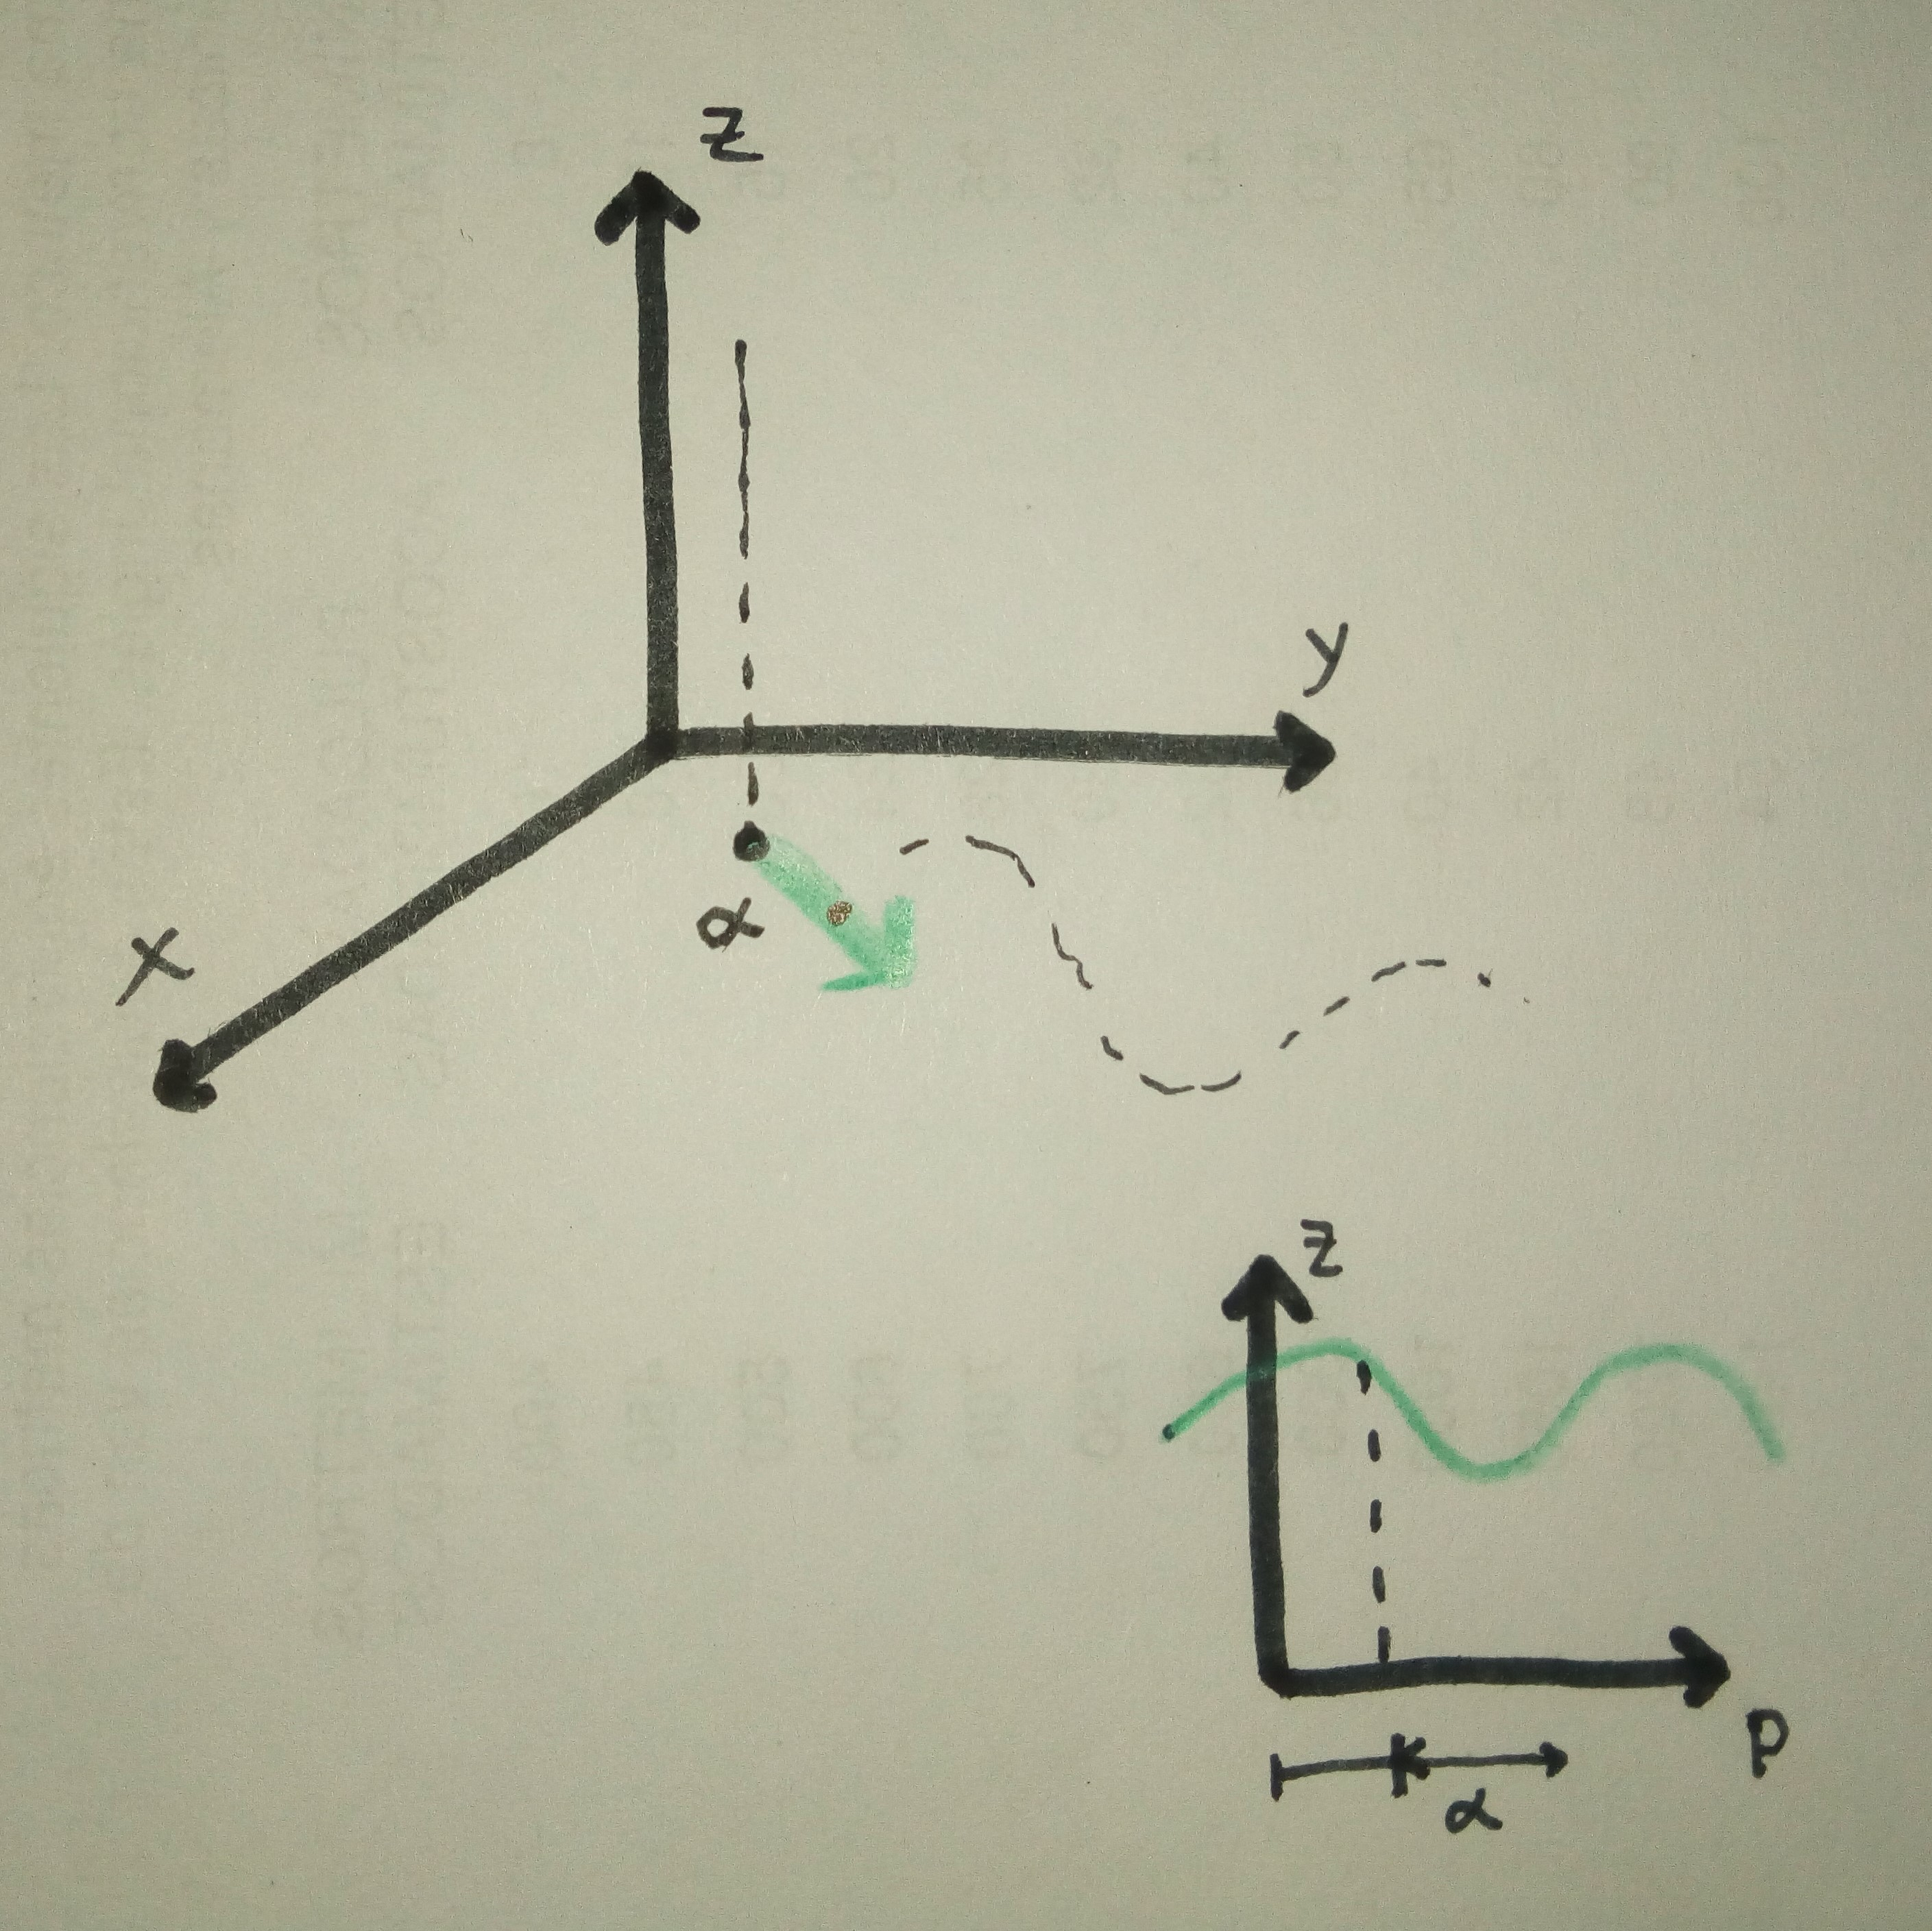
\includegraphics[scale=.05]{imagenes/7.jpg}
\end{center}

\subsubsection*{Tecnicas de precondicionamiento}

$Ax=b$\\
$\hat{x}=Cx$ Donde $C$ es la matriz de rotaci\'on \\
$x=C^{-1}\hat{x}$\\
$C^{-T}AC^{-1}\hat{x}=C^{-T}b$

\subsubsection{Gradiente Conjugado con precondicionamiento de Jacobi}
%Solo el algoritmo%
\subsection{Gradiente biconjugado}
\begin{center}
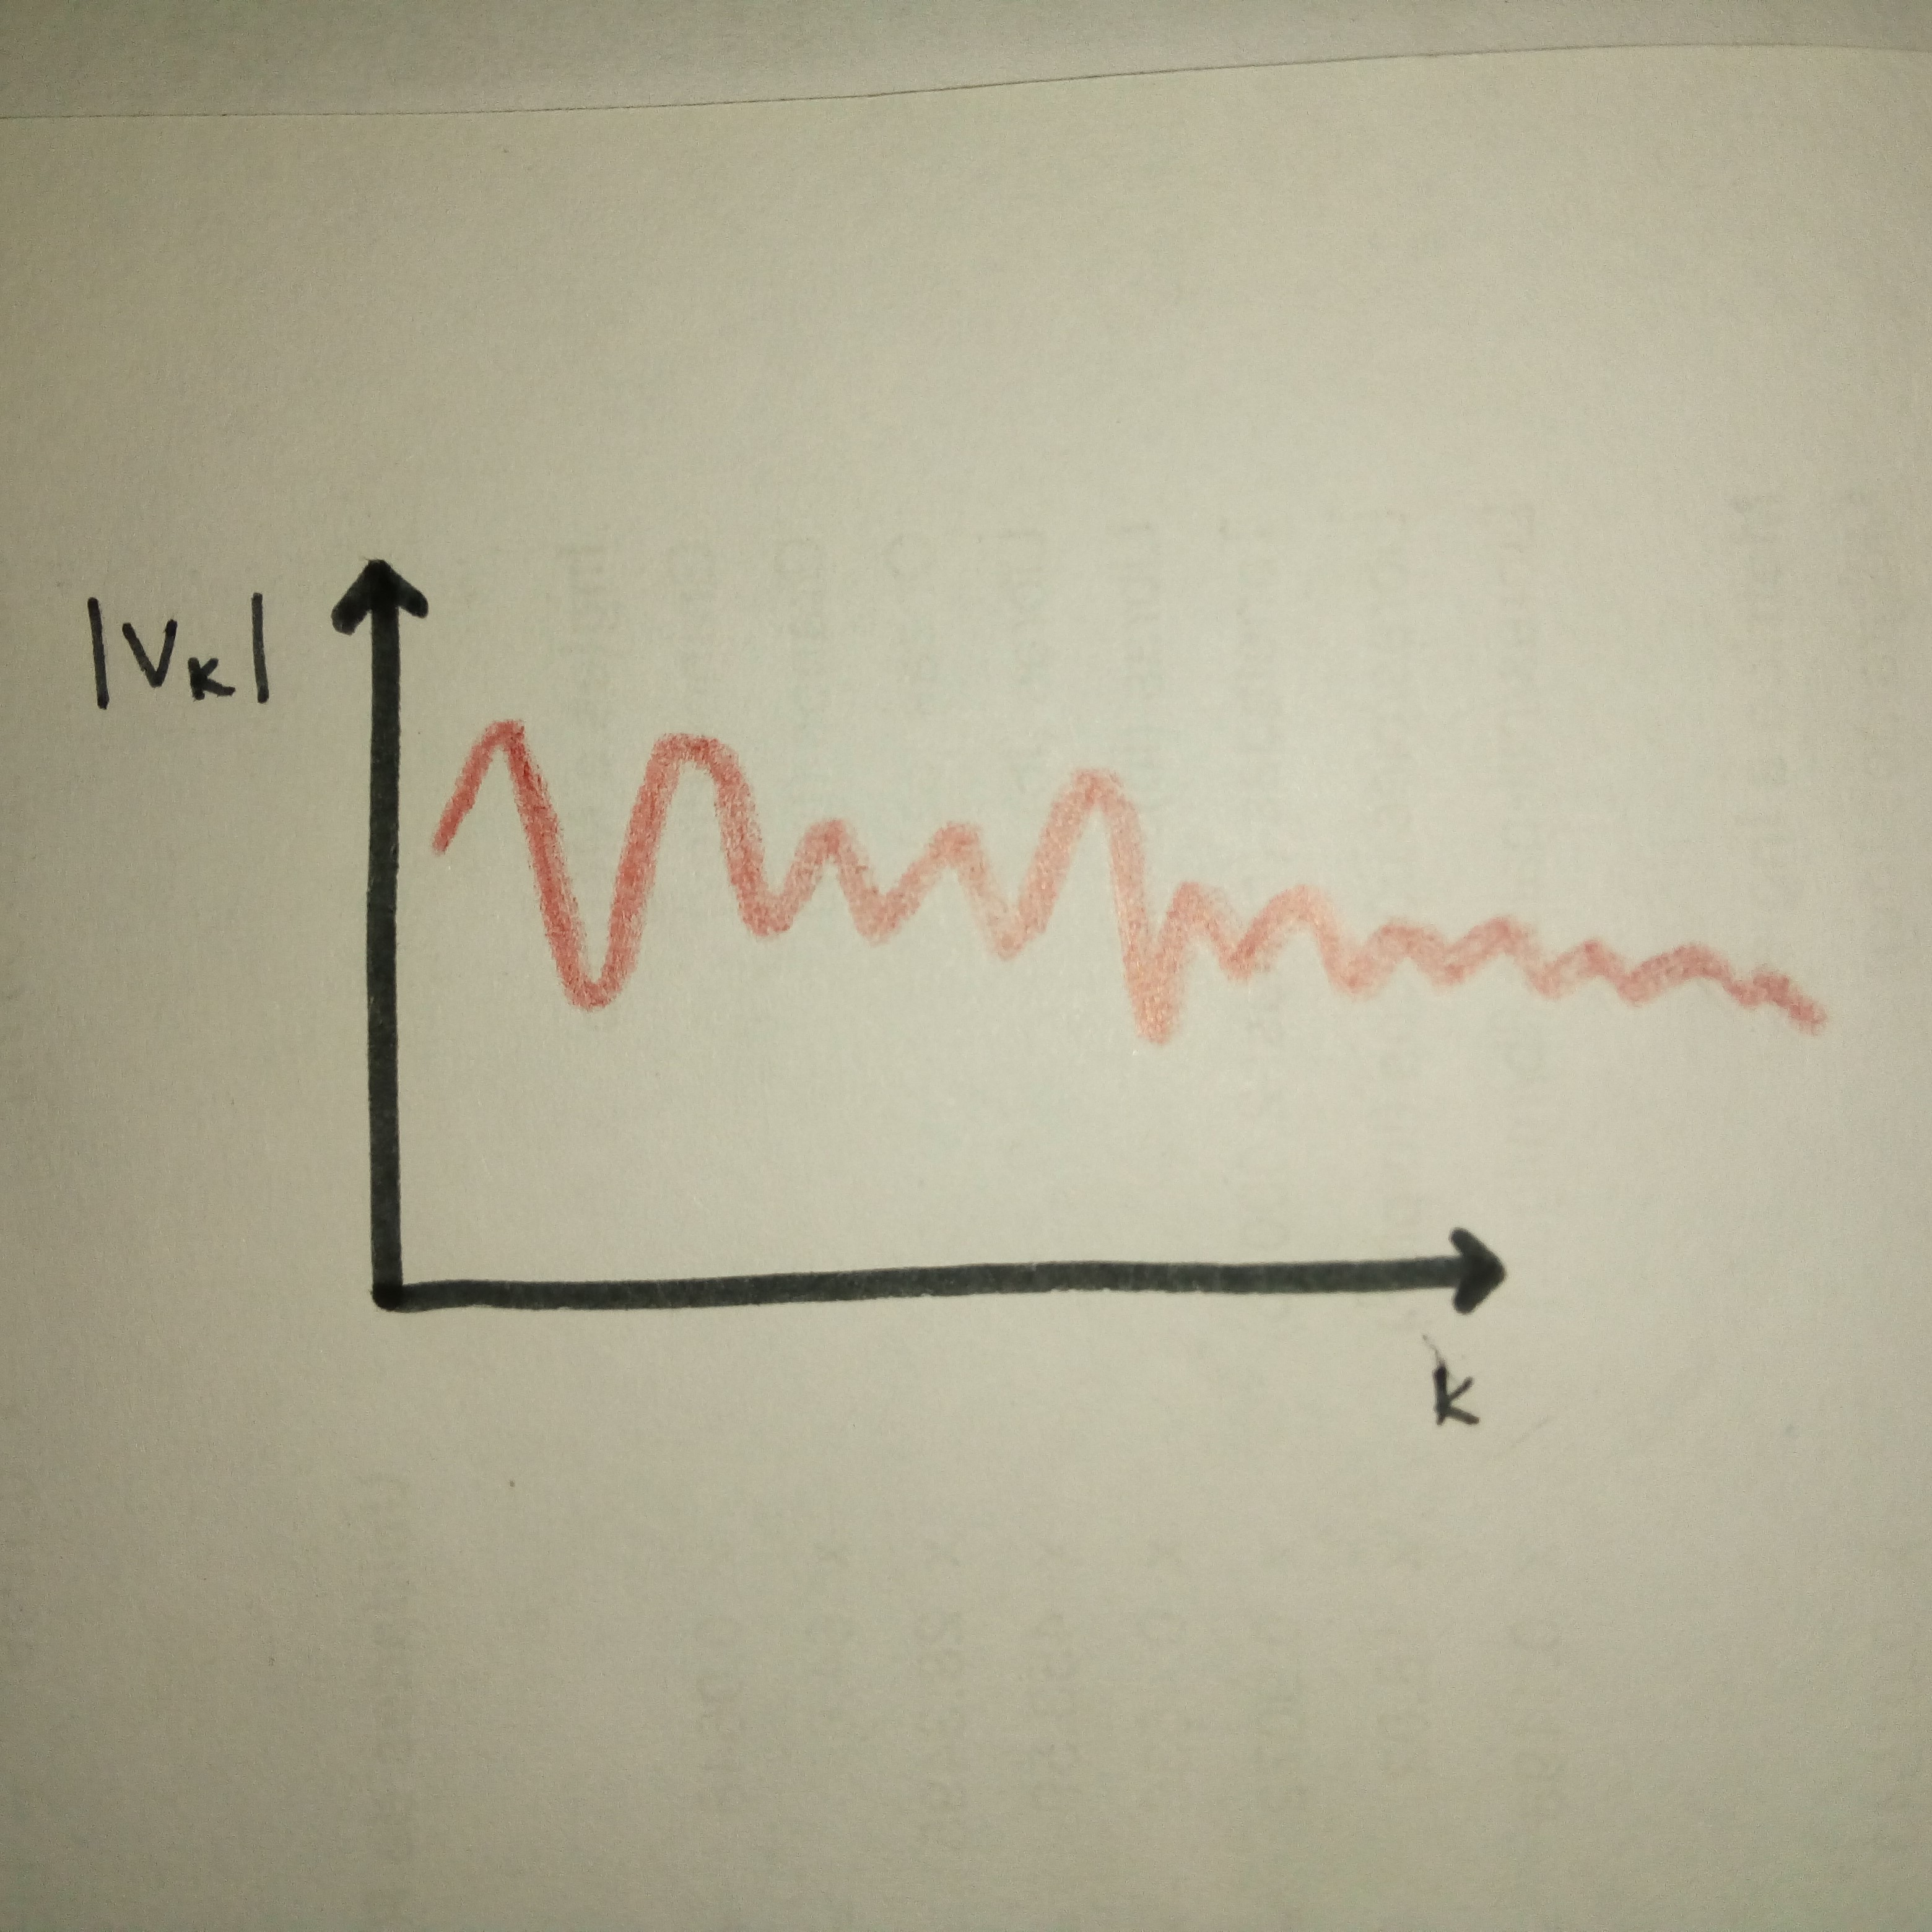
\includegraphics[scale=.05]{imagenes/8.jpg}
\end{center}
\subsection{Gradiente conjugado cuadrado}
%solo algoritmo%